\documentclass[a4paper,11pt]{book}
\usepackage{listings}
\usepackage[utf8]{inputenc}
\usepackage{titlesec}
\usepackage{fancyhdr}
\usepackage[spanish,es-tabla]{babel}
\usepackage[hidelinks]{hyperref}
\usepackage{xcolor}
\usepackage{pdfpages}

% Información reutilizable
\newcommand{\asunto}{Trabajo de Fin de Grado}
\newcommand{\titulo}{Observatorio Remoto: un cliente INDI para Android}
\newcommand{\tituloEng}{Remote Observatory: A INDI client to Android}
\newcommand{\grado}{Grado en Ingeniería Informática}
\newcommand{\autor}{Jaime Torres Benavente}
\newcommand{\email}{jtbenavente@gmail.com}
\newcommand{\tutor}{Sergio Alonso Burgos}
\newcommand{\escuela}{Escuela Técnica Superior de Ingenierías Informática y de Telecomunicación}
\newcommand{\universidad}{Universidad de Granada}
\newcommand{\ciudad}{Granada}
\newcommand{\vers}{Versión 1.0}

% Información archivo
\hypersetup{
	pdfauthor = {\autor\ (\email)},
	pdftitle = {\titulo},
	pdfsubject = {\asunto},
	pdfkeywords = {software libre, INDI, astronomía, Android, telescopio, CCD},
	pdfcreator = {LaTeX con el paquete texlive},
	pdfproducer = {pdflatex}
}

% Estilo de cabeceras
\pagestyle{fancy}
\fancyhf{}
\fancyhead[LO]{\leftmark}
\fancyhead[RE]{\rightmark}
\fancyhead[RO,LE]{\textbf{\thepage}}
\setlength{\headheight}{1.5\headheight}

% Redefinición de comandos
\renewcommand{\lstlistingname}{Fragmento de código}
\renewcommand{\lstlistlistingname}{Índice de fragmentos de código}
\renewcommand{\chaptermark}[1]{\markboth{\textbf{#1}}{}}
\renewcommand{\sectionmark}[1]{\markright{\textbf{\thesection. #1}}}

% Definición de colores
\definecolor{gray97}{gray}{.97}
\definecolor{gray75}{gray}{.75}
\definecolor{gray45}{gray}{.45}
\definecolor{gray30}{gray}{.94}
\definecolor{lightgray}{rgb}{.9,.9,.9}
\definecolor{darkgray}{rgb}{.4,.4,.4}
\definecolor{purple}{rgb}{0.65, 0.12, 0.82}
\definecolor{background}{HTML}{EEEEEE}
\definecolor{delim}{RGB}{20,105,176}
\colorlet{punct}{red!60!black}
\colorlet{numb}{magenta!60!black}

% Listados
\lstset{
	aboveskip=0.5cm,
	backgroundcolor=\color{gray97},
	basicstyle=\scriptsize\ttfamily,
	breaklines=true,
	commentstyle=\color{gray45},
	frame=Ltb,
	framerule=0.5pt,
	framesep=0pt,
	framexbottommargin=3pt,
	framexleftmargin=0.1cm,
	framextopmargin=3pt,
	keywordstyle=\bfseries,
	numberfirstline = false,
	numbers=left,
	numbersep=6pt,
	numberstyle=\tiny,
	rulesep=.4pt,
	rulesepcolor=\color{black},
	showstringspaces = false,
	stringstyle=\ttfamily,
	literate={á}{{\'a}}1
	         {é}{{\'e}}1
	         {í}{{\'i}}1
	         {ó}{{\'o}}1
	         {ú}{{\'u}}1
	         {ñ}{{\~n}}1
}
 
% Minimizar fragmentado de listados
\lstnewenvironment{listing}[1][]
	{\lstset{#1}\pagebreak[0]}{\pagebreak[0]}

% Listado definido para JavaScript
% http://tex.stackexchange.com/questions/89574/language-option-supported-in-listings/89576#89576
\lstdefinelanguage{javascript}{
	backgroundcolor=\color{background},
	basicstyle=\footnotesize,
	breaklines=true,
	captionpos=b,
	comment=[l]{//},
	commentstyle=\color{purple}\ttfamily,
	frame=lines,
	identifierstyle=\color{black},
	keywordstyle=\color{blue}\bfseries,
	morecomment=[s]{/*}{*/},
	morestring=[b]',
	morestring=[b]",
	ndkeywordstyle=\color{darkgray}\bfseries,
	numbers=left,
	numbersep=8pt,
	numberstyle=\scriptsize,
	sensitive=false,
	showstringspaces=false,
	stepnumber=1,
	stringstyle=\color{red}\ttfamily,
	keywords={
		break,
		case,
		catch,
		catch,
		do,
		else,
		false,
		function,
		if,
		in,
		new,
		null,
		return,
		switch,
		true,
		typeof,
		var,
		while},
	ndkeywords={
		boolean,
		class,
		export,
		implements,
		import,
		this,
		throw}
}

% Listado definido para JSON
% http://tex.stackexchange.com/questions/83085/how-to-improve-listings-display-of-json-files/83100#83100
\lstdefinelanguage{json}{
	backgroundcolor=\color{background},
	basicstyle=\footnotesize,
	breaklines=true,
	captionpos=b,
	frame=lines,
	numbers=left,
	numbersep=8pt,
	numberstyle=\scriptsize,
	showstringspaces=false,
	stepnumber=1,
	literate=
		*{:}{{{\color{punct}{:}}}}{1}
		{,}{{{\color{punct}{,}}}}{1}
	    {\{}{{{\color{delim}{\{}}}}{1}
	    {\}}{{{\color{delim}{\}}}}}{1}
	    {[}{{{\color{delim}{[}}}}{1}
	    {]}{{{\color{delim}{]}}}}{1}
	    {ñ}{{\~{n}}}{1}
}

% Para que las páginas en blanco no tengan cabecera
\makeatletter
\def\clearpage{%
  \ifvmode
    \ifnum \@dbltopnum =\m@ne
      \ifdim \pagetotal <\topskip
        \hbox{}
      \fi
    \fi
  \fi
  \newpage
  \thispagestyle{empty}
  \write\m@ne{}
  \vbox{}
  \penalty -\@Mi
}
\makeatother

\begin{document}
\begin{titlepage}

\newlength{\centeroffset}
\setlength{\centeroffset}{-0.5\oddsidemargin}
\addtolength{\centeroffset}{0.5\evensidemargin}

\noindent\hspace*{\centeroffset}\begin{minipage}{\textwidth}

\centering

\includegraphics[width=0.9\textwidth]{../images/logo_ugr.png}\\[1.4cm]

\textsc{\Large\asunto\\[0.2cm]}
\textsc{\grado}\\[1cm]

{\Huge\bfseries \titulo\\}
\noindent\rule[-1ex]{\textwidth}{3pt}\\[3.5ex]
\end{minipage}

\vspace{2cm}
\noindent\hspace*{\centeroffset}\begin{minipage}{\textwidth}
\centering

\textbf{Autor}\\ {\autor}\\[2.5ex]
\textbf{Tutor}\\ {\tutor}\\[2cm]

\includegraphics[width=0.3\textwidth]{../images/logo_etsiit.png}\\[0.1cm]
\textsc{\escuela}\\
\textsc{---}\\
\ciudad, \today\\

\includegraphics[width=0.3\textwidth]{../images/CC-SA-logo.png}
\end{minipage}
\end{titlepage}
\frontmatter
\begin{center}
{\LARGE\bfseries\titulo}\\
\end{center}
\begin{center}
\autor\
\end{center}

\newpage
\thispagestyle{empty}
\
\vspace{3cm}

\noindent\rule[-1ex]{\textwidth}{2pt}\\[4.5ex]

Yo, \textbf{\autor}, alumno de la titulación \textbf{\grado} de la \textbf{\escuela\ de la \universidad}, autorizo la ubicación de la siguiente copia de mi Trabajo Fin de Grado (\textit{\titulo}) en la biblioteca del centro para que pueda ser consultada por las personas que lo deseen.

\bigskip
Además, este mismo trabajo es realizado bajo licencia \textbf{Creative Commons Attribution-ShareAlike 4.0} (\url{https://creativecommons.org/licenses/by-sa/4.0/}), dando permiso para copiarlo y redistribuirlo en cualquier medio o formato, también de adaptarlo de la forma que se quiera, pero todo esto siempre y cuando se reconozca la autoría y se distribuya con la misma licencia que el trabajo original. El documento en formato {\tt LaTeX} así como el código del proyecto se puede encontrar en el siguiente repositorio de {\tt GitHub}: \url{https://github.com/torresj/indi-android-ui}.

\vspace{4cm}

\noindent Fdo: \autor

\vspace{2cm}

\begin{flushright}
\ciudad, a \today
\end{flushright}

\newpage
\thispagestyle{empty}
\
\vspace{3cm}

\noindent\rule[-1ex]{\textwidth}{2pt}\\[4.5ex]

D. \textbf{\tutor}, profesor del \textbf{Departamento de Lenguajes y Sistemas Informáticos} de la \textbf{\universidad}.

\vspace{0.5cm}

\vspace{0.5cm}

\textbf{Informa:}

\vspace{0.5cm}

Que el presente trabajo, titulado \textit{\textbf{\titulo}}, ha sido realizado bajo su supervisión por \textbf{\autor}, y 
autoriza la defensa de dicho trabajo ante el tribunal que corresponda.

\vspace{0.5cm}

Y para que conste, expide y firma el presente informe en \ciudad\ a \today.

\vspace{1cm}

\textbf{El tutor:}

\vspace{5cm}

\noindent \textbf{\tutor}

\chapter*{Agradecimientos}
\thispagestyle{empty}

\vspace{1cm}

A mi familia porque gracias a ellos soy como soy.

\bigskip
A mis amigos porque sin ellos no habría podido llegar hasta aquí

\bigskip
A mi tutor \textbf{\tutor}, por aguantarme durante tantos meses con una paciencia infinita.


\begingroup
\let\cleardoublepage\clearpage
  \tableofcontents
  \listoffigures
  \listoftables
  \lstlistoflistings
\endgroup

\newpage
\thispagestyle{empty}
\
\mainmatter
\chapter{Introducción}

\section{La Astronomía}

Desde el princpio de los tiempos, el ser humano a mirado al cielo con incertidumbre, viendolo como una fuente inagotable de interrogantes sin resolver. En casi todas las religiones antiguas existía la \textbf{``cosmogonía''} que intentaba explicar el origen del universo, ligando este a los elementos mitológicos, dando paso esta a la \textbf{``astronomía''}:

\begin{quote}``\textit{Ciencia que se ocupa del estudio de los cuerpos celestes del universo, incluidos los planetas y sus satélites, los cometas y meteorítos, las estrellas y la materia interestelar, los sistemas de materia oscura, estrellas, gas y polvo llamados galaxias y los cúmulos de galaxias; por lo que estudia sus movimientos y fenómenos ligaods a ellos.}''
\newline(\url{https://es.wikipedia.org/wiki/Astronom%C3%ADa})
\end{quote}

\bigskip
 La Astronomía es probablemente la más antigua de las ciencias naturales originándose en la antiguedad en casi todas las culturas humanas. Sus orígenes se pierden en prácticas religiosas de la prehistoria cuyos vestigios se encuentran en numerosos sitios arqueológicos (como Stonehenge) e incorporados todavía en la astrología una disciplina entrelazada con la astronomía y no separada de ella completamente hasta el siglo XVIII en el mundo occidental. La astronomía antigua constituyó las bases del calendario y la medida de periodos temporales como la semana el mes o el año. Los astrónomos antiguos eran capaces de distinguir entre estrellas y planetas dado que las primeras permanecen fijas en sus posiciones relativas mientras que los planetas se mueven una cantidad apreciable de espacio a lo largo de periodos relativamente cortos ( Saturno el más lento de los planetas conocidos en la antigüedad describe un periodo orbital en 29 años). La Astronomía antigua culmina con el desarrollo ordenado del modelo heliocéntrico expuesto en las obras de \textit{Ptolomeo}. Previamente \textit{Aristarco de Samos} había medido las distancias de la Tierra a la Luna y al Sol afirmando como consecuencia de éstas que el Sol era el centro del Universo alrededor del cual giraban los demás planetas incluyendo la Tierra. Otros logros destacados de la época clásica de la astronomía fueron los conseguidos por \textit{Hiparco} quien realizó el primer catálogo estelar y propuso un sistema de clasificación estelar en 6 magnitudes basado en la luminosidad aparente de las diferentes estrellas. La Astronomía en la Europa medieval se produce un oscurantismo en todos los campos del conocimiento incluyendo la astronomía. Ésta permanece preservada en escasas copias de tratados antiguos de la astronomía griega y romana. La astronomía observacional tan sólo se conserva en el mundo árabe.

 \bigskip
 \textit{Tycho Brahe (1546-1601)} introdujo la idea de la precisión de la medida en astronomía e inventó y produjo una gran cantidad de instrumental astronómico previo al telescopio. \textit{Galileo Galilei (1564-1642)} construyó su propio telescopio a partir de un invento holandés y lo utilizó inmediatamente en el estudio astronómico descubriendo los cráteres de la Luna, las lunas de Júpiter y las manchas solares. Sus observaciones tan sólo eran compatibles con el modelo \textbf{copernicano}. Paralelamente \textit{Johannes Kepler} expuso sus famosas \textbf{leyes de Kepler} para el movimiento de los planetas basándo su trabajo en las detalladas observaciones de \textit{Tycho Brahe}.

\bigskip
Una generación más tarde Isaac Newton fue el primer científico que unió la Física con la Astronomía proponiendo que las mismas fuerzas que hacían caer los cuerpos sobre la Tierra causaban el movimiento de los planetas y la Luna. Utilizando su Ley de la gravedad las leyes de Kepler resultan inmediatamente explicadas. Newton también descubrió que la Luz blanca del Sol está descompuesta en diferentes colors, un hecho importantísimo para el futuro desarrollo de la astronomía.

\bigskip
La \textbf{astronomía} es una de las pocas ciencias en las que los aficionados aún puden desempeñar un papel activo, especialmente en el descubirmientos y seguimiento de fenómenos. Es por ello que existe una gran variedad de \textbf{herramientas} e \textbf{instrumental astronómico} que permiten a cualquier persona obervar el universo.

\newpage
\section{Instrumental Astronómico}

Existe una gran variedad de \textbf{instrumental astronómico} en la actualidad. A continuación se describen las familias más importantes.

\subsection{Telescopios}

\begin{quote}``\textit{El telescopio es un instrumento óptico que permite ver objetos lejanos con mucho más detalle que a simple vista al captar radiación electromagnética, tal como la luz.}''
\newline(\url{https://es.wikipedia.org/wiki/Telescopio})
\end{quote}

\bigskip
Hace cuatro siglos nació un invento que habría de redefinir nuestro lugar en el universo. Tachado en su momento como el instrumento más diabólico de la historia, el telescopio sacudió la sociedad hasta las raíces. Al alzar los ojos al cielo nos convencimos de que éramos el centro de la creación, y había razones para ello: desde nuestra perspectiva, todo parece girar en torno a la Tierra

\bigskip
Los fabricantes de vidrio sabían desde la antigüedad que una esfera de vidrio podía aumentar imágenes, pero tuvieron que pasar siglos antes de que alguien ensamblara dos lentes en un tubo y mirara a través de ellas. Señalar la fecha, lugar y autor exactos de su invención es controvertido. Los holandeses se inclinan por el 2 de octubre de 1608, el día en que \textit{Hans Lippershey} patentó un instrumento llamado \textbf{kijker}, que significa mirador. Un moledor de vidrio holandés aseguraba haber inventado un aparato similar, pero el primero en patentarlo fue \textit{Lippershey}. Como era alemán, vivía en Holanda y registró la patente en Bélgica, más de un país ha pugnado por el honor de su autoría. Sin embargo, como dijo \textit{Darwin}:
\begin{quote}``\textit{en la ciencia el crédito es del que convence al mundo y no del primero en tener la idea}''
\newline(\textbr{Charles Darwin})
\end{quote}
Por eso la gloria se la llevó Italia, ya que fueron las mejoras que introdujo \textit{Galileo} las que permitieron usar el aparato como instrumento astronómico. El diseño de \textit{Galileo} consistía en una lente convexa para el objetivo y otra cóncava en el ocular. En 1611 el alemán \textit{Johannes Kepler} fue el primero en usar dos lentes convexas que enfocaban los rayos en un mismo punto. La configuración de \textit{Kepler} aún se usa en binoculares y cámaras fotográficas modernas y es la base del telescopio refractor.

\bigskip
Tras la muerte de \textit{Galileo}, fue \textit{Isaac Newton} quien nos dio una nueva imagen del universo que sobrevivió 250 años hasta la llegada de \textit{Albert Einstein}.

\begin{quote}``\textit{Si he logrado ver más lejos ha sido porque me he subido a hombros de gigantes}''
\newline(\textbf{Isaac Newton})
\end{quote}

Y así, sobre la herencia de \textit{Galileo}, \textit{Newton} inventó el \textbf{telescopio reflector}, que es la base de los actuales. La innovación consistía en usar espejos en lugar de lentes para enfocar la luz y formar imágenes. Entonces el universo se nos abrió en todo su esplendor.

\subsection{Cámaras CCD}

Un dispositivo de carga acoplada (en inglés \textbf{Charge-Coupled Device}, conocido también como \textbf{CCD}), es un circuito integrado que contiene un número determinado de condensadores enlazados o acoplados. Bajo el control de un circuito interno, cada condensador puede transferir su carga eléctrica a uno o a varios de los condensadores que estén a su lado en el circuito impreso.

\bigskip
El \textbf{CCD} se inventó a finales delos 60 por investigadores de \textbf{Bell Laboratories}. Originalmente se concibió como un nuevo tipo de memoria de ordenador pero pronto se observó que tenía muchas más aplicaciones potenciales tales como el proceso de señales y sobretodo la captación de imagen, esto último debido a la sensibilidad a la luz que presenta el silicio.

\bigskip
El sensor \textbf{CCD} de una cámara digital es como el motor de un coche, es la pieza principal. En su forma más elemental, el \textbf{CCD} es como un ojo electrónico que recoje la luz y la convierte en una señal eléctrica. Tienen dos diferencias básicas con los fotomultiplicadores:

\bigskip
Los sensores \textbf{CCD} son de menor tamaño y están construidos de semiconductores lo que permite la integración de millones de dispositivos sensibles en un solo chip.
La eficiencia cuóntica de los \textbf{CCD} (sensibilidad) es mayor para los rojos. Los fotomultiplicadores son más sensibles a los azules.

\bigskip
Físicamente, un \textbf{CCD} es una malla muy empaquetada de electrodos de polisilicio colocados sobre la superficie de un chip. Al impactar los fotones sobre el silicio se generan electrones generados que pueden guardarse temporalemte. Periódicamente se lee el contenido de cada pixel haciendo que los electrones se desplacen físicamente desde la posición donde se originaron (en la superficie del chip), hacia el amplificador de señal con lo que se genera una corriente eléctrica que será proporcional al número de fotones que llegaron al pixel. Para coordinar los periodos de almacenamiento (tiempo de exposición) y vaciado del pixel (lectura del pixel) debe existir una fuente eléctrica externa que marque el ritmo de almacenamiento-lectura: el reloj del sistema. La forma y amplitud de reloj son críticas en la operación de lectura del contenido de los pixeles.

\bigskip
Al tratarse el \textbf{CCD} de un dispositivo semiconductor, técnicamente es posible implementar en él todas las funciones electrónicas de un sistema de captación de imagen, pero esto no es rentable económicamente y por tanto se implementa en otros chips esternos al \textbf{CCD}: la mayoría de \textbf{CCD} de cámaras tienen varios chips (de tres a ocho).

\bigskip
La necesidad de usar chips distintos implica dos desventajas importantes; la necesidad de voltajes múltiples de abastecimiento de los chips y un gran consumo de potencia de todo el sistema electrónico.

\subsection{Monturas}

La montura de un telescopio es la parte mecánica que une el trípode o base al instrumento óptico. Existen varios tipos de monturas, algunas muy simples, otras mas complejas, incluso con correctores electrónicos y dispositivos de localización y seguimiento muy sofisticados (sistenas \textbf{GOTO})

\bigskip
La montura tiene como objetivo proveer de movimiento controlado al telescopio. Es muy importante la firmeza y suavidad de los movimientos, para que la observación sea confortable y las astrofotografías perfectas. Las monturas se clasifican en dos grandes grupos, según los planos de referencia que utilicen (coordenadas).

\bigskip
La más simple es la montura altacimutal, que realiza movimientos horizontales y verticales (acimut y altura, respectivamente). Este tipo de diseño lo traen incorporados los telescopios pequeños, por lo general telescopios refractores de uso terrestre, dado que su uso es simple, y también varios modelos de equipos automatizados (sistemas \textbf{GOTO})

\bigskip
Le sigue la montura ecuatorial, que utiliza como plano fundamental el ecuador celeste (proyección del ecuador terrestre). Este diseño usa las coordenadas ecuatoriales, ascensión recta (A.R. o R.A.) y declinación (Dec.), que son proyecciones de las coordenadas terrestres longitud y latitud, respectivamente, sobre la esfera celeste.

\bigskip
Existen varios tipos de monturas basados en los dos diseños fundamentales anteriores. La montura \textbf{Dobson} por ejemplo (suelen llamarse telescopios \textit{dobsonianos} a los que la poseen), es un modelo basado en la altacimutal, sin trípode y un telescopio de diseño newtoniano como instrumento de observación. Es muy utilizado por los que desean una gran apertura en reflectores, por ejemplo los que se construyen su propio espejo y no quieran tener grandes gastos en monturas sofisticadas.

\subsection{Rueda portafiltro}

La rueda porta-filtros consiste en un cuerpo, generalmente de aluminio, que en su interior puede alojar varios filtros, normalmente de 1,25" de diámetro. Lo aconsejable es que tenga, al menos, 4 huecos para filtros si queremos hacer astrofotografía con cámaras CCD blanco y negro, puesto que vamos a necesitar el azul, rojo y verde (RGB) y, posiblemente, un filtro para infrarrojos.

\subsection{Enfocadores}

El \textbf{enfocador} es una pieza fundamental del telescopio. Nos permitirá ver las imágenes formadas tras la reflexión de la luz en el espejo primario y su desviación por el espejo secundario. Para verlas necesitaremos un juego de oculares. La longitud focal de los oculares combinada con la longitud focal de nuestro telescopio nos dará el número de aumentos total del sistema. Dichos oculares están montados en el \textbf{enfocador}, un dispositivo móvil que permitirá mover la posición vertical del ocular para enfocar adecuadamente la imagen.

\bigskip
Un ejemplo de enfocador son los de tipo \textbf{Crayford} y los \textbf{rack and pinion}.

\subsection{Cúpulas}
Las \textbf{cúpulas} son recintos cerrados mas o menos grandes que nos permiten albergar y proteger el instrumental astronómico. De esta forma, las \textbf{cúpulas} pueden ser abiertas o cerradas para exponer los instrumentos en el momento de las observaciones.

\subsection{Ópticas adaptativas}

La \textbf{óptica adaptativa} es una técnica que permite corregir las perturbaciones más importantes que sufren las imágenes astronómicas debido a la atmósfera terrestre. Con este sistema es posible obtener imágenes más nítidas o de mejor resolución espacial. La diferencia que introduce esta técnica es comparable a la que existe entre mirar un objeto situado en el fondo de una piscina con agua o sin agua.

\bigskip
Las posibilidades que la óptica adaptativa ofrece a la astronomía son espectaculares. Eliminar las perturbaciones producidas por la atmósfera equivale esencialmente a observar desde el espacio. Las perturbaciones atmosféricas causan una pérdida en nitidez o resolución espacial. Esta pérdida se traduce, por un lado, en una disminuida capacidad para resolver objetos, es decir, para realizar estudios detallados de su morfología. Por otro lado, influye también en la capacidad de detectar objetos débiles, dado que la imagen se dispersa en puntos de luz mayores.

\bigskip
La mejora que introduce la óptica adaptativa se puede cuantificar utilizando la relación entre el tamaño del telescopio y el tamaño de la mejor imagen que puede obtener. El poder de detección de un telescopio aumenta con el diámetro de su espejo primario y disminuye con el tamaño de la imagen que forma de un objeto puntual (de aquí la importancia de la calidad de imagen en un telescopio). Por tanto, la diferencia con un mismo espejo de 10 metros, entre conseguir enfocar imágenes de 0.4 segundos de arco (lo posible en una noche de visibilidad excelente) y una imagen de 0.04 segundos de arco, que debe ser posible con un sistema de óptica adaptativa, equivaldría a tener un espejo primario de 100 metros

\subsection{Estaciones meteorológicas}

Las \textbf{estaciones meteorológicas} son sistemas compuestos por un \textit{``data logger''} y un conjunto de sensores que nos proprcionan datos de las distintas magnitudes meteorolóygicas, tales como la temperatura, humedad, presión barométrica, etc... permitiéndonos generar modelos a partir de los cuales conocer la situación climática y su posible evolución. 

\bigskip
Gracias a los datos aportados por las \textbf{estaciones meteorológicas}, podemos conocer la climatología en el momento de realizar observaciones astronómicas. De esta forma podemos decidir si las condiciones son óptimas, o incluso decidir si debemos cerrar la cúpula para evitar daños en los intrumentos por lluvias o similar. 

\newpage
\section{Control de dispositivos astronómicos}

Actualmente existen diversas formas de controlar los dispositivos astronómicos pero la mayoría presenta los mismos incovenientes:

\begin{itemize}
  \item Normalmente se controlan los dispositivos directamente.
  \item Se conecta el dispositivo a un PC y se trabaja desde él.
  \item Se utilizan herramientas para el control remoto como el \textif{``escritorio remoto''}.
\end{itemize}

\bigskip

Por otro lado, existen estándares como el de \textbf{ASCOM} para instrumental astronómico. Con él, se intenta crear una capa entre los programas para controlar dispositivos astronómicos y los propios dispositivos. La principal desventaja es que solo puede utilizarse en sistemas \textit{Microsoft Windows}

\bigskip
\begin{figure}[!ht]
  \begin{center}
    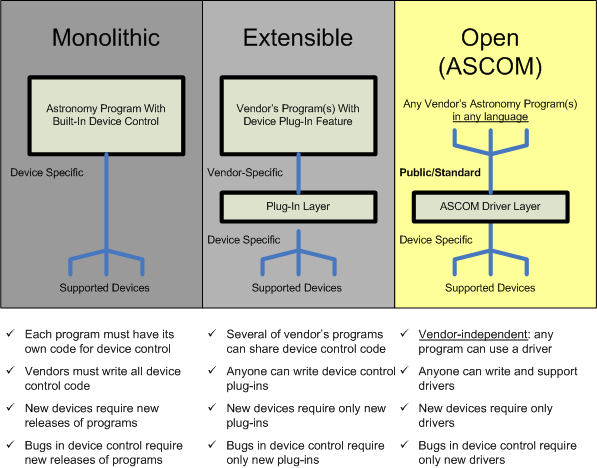
\includegraphics[scale=0.5]{../images/ascom.png}
    \caption{ASCOM Standard (\url{http://ascom-standards.org/})}
    \label{fig:ascom}
  \end{center}
\end{figure}


\newpage
\section{INDI}

\begin{quote}``\textit{The Instrument Neutral Distributed Interface (INDI) Library is a cross-platform software designed for automation & control of astronomical instruments. It supports a wide variety of telescopes, CCDs, focusers , filter wheels..etc, and it has the capability to support virtually any device. INDI is small, flexible, easy to parse, and scalable. It supports common DCS functions such as remote control, data acquisition, monitoring, and a lot more. With INDI, you have a total transparent control over your instruments so you can get more science with less time.}''
\newline(\url{http://indilib.org/about.html})
\end{quote}

\bigskip

El protocolo \textbf{INDI} es una plataforma software diseñada para el control de instrumental astronómico. La biblioteca \textbf{INDI} permite controlar cualquier dispositivo con un driver \textbf{INDI} mediante el paso de archivos XML. Sus principales ventajas frente a otras soluciones para el control de dispositivos son:


\begin{itemize}
  \item Es una biblioteca ligera, flexible y escalable.
  \item Es de código abierto por lo que cualquiera puede ver su código y mejorarlo o crear drivers para cualquier dispositivo
  \item El intercambio de información es mínimo.
  \item Es multiplataforma.
  \item Separa el cliente del servidor.
  \item Los fabricantes comienzan a desarrollar drivers para sus dispositivos o liberan las especificaciones para que la comunidad pueda desarrollarlos.
  \item Existen numerosos clientes INDI como \url{https://edu.kde.org/kstars/}

\end{itemize}

\bigskip
\begin{figure}[!ht]
  \begin{center}
    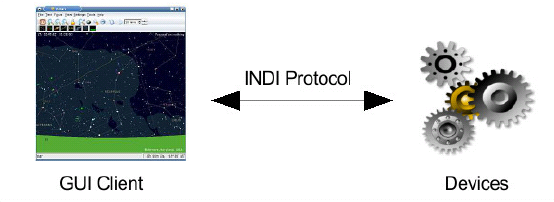
\includegraphics[width=1\textwidth]{../images/Indi_client.png}
    \caption{INDI Client (\url{http://www.indilib.org/})}
    \label{fig:indi_client}
  \end{center}
\end{figure}

\bigskip
\begin{figure}[!ht]
  \begin{center}
    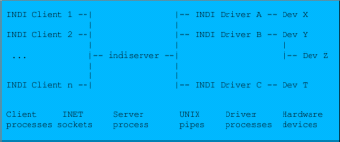
\includegraphics[width=1\textwidth]{../images/Indi_server.png}
    \caption{INDI Server (\url{http://www.indilib.org/})}
    \label{fig:indi_server}
  \end{center}
\end{figure}

\bigskip

\subsection{INDI for Java}

La biblioteca \textbf{INDI} está escrita en lenguaje \textbf{C}, pero existe una implementación realizada en Java y que se encuentra en desarrollo. En la página oficial de \textbf{INDI} \url{http://indilib.org/develop/indiforjava.html} podemos encontrar toda la información sobre nuevas versiónes y la documentación para poder utilizarla. La principal ventaja de poder usar Java es que podemos implementar drivers y clientes con la potencia de un lenguaje Orientado a Objetos y combinarlo con otras tecnologías como los dispositivos móviles basados en la plataforma \textbf{Android}


\newpage

\section{Dispositivos Móviles}

Un \textbf{dispositivo móvil} es un tipo de computadora de tamaño pequeño, con capacidad de procesamiento, con conexión a internet, con memoria, diseñados especifcamente para una función pero que pueden llevar a cabo otras funciones más generales.

\bigskip
Los \textbf{dispositivos móviles} hoy en día están integrados en la mayoría de tareas cotidianas de una persona. La tendencía de la sociedad actual nos empuja hacia un mundo cada vez más móvil donde necesitamos estar conectado e interactuar con otros sitemas. Es por ello que la mayoría de soluciones tecnológicas, hayan sido pensadas o no para el sector de los dispositivos móviles, siempre acaba teniendo una versión para éstos.

\bigskip
Paralelamente a la expansión de los \textbf{dispositivos móviles}, se han creado un gran número de sistemas operativos para estos dispositivos entre los que se encuentra:

\begin{itemize}
  \item Android.
  \item iOS.
  \item BlackBerry OS.
  \item Palm OS.
  \item Windows Mobile/Phone.
  \item Symbian.
\end{itemize}

\bigskip
Actualmente \textbf{Android} y \textbf{iOS} copan el 96.3\% del mercado\footnote{Fuente:http://www.idc.com/getdoc.jsp?containerId=prUS25450615.} . Por lo que nos centraremos principalmente en estos S.O.\footnote{Sistema Operativo.} y los \textbf{dispositivos móviles} compatibles con ellos.

\subsection{iOS}

\textbf{iOS} es un S.O. móvil de la compaía \textit{Apple Inc} originalmente desarrollado para el \textit{iPhone}\footnote{Smartphone de la compañia Apple Inc.} y posteriormente introducido en otros \textbf{dispositivos móviles} de la compañía como el iPod touch\footnote{Dispositivo móvil para reproducir multimedia de la compañía Apple Inc} y el iPad\footnote{Tablet de la compañía Apple Inc.}. \textbf{iOS} no puede ser instalado en hardware de terceros.

\bigskip
Actualmente tiene una cuota de mercado aproximadamente del 19.7\%, siendo el segundo S.O. más utilizado.

\bigskip
\textbf{iOS} es un sistema muy estable, diseñado para un hardware muy concreto y por tanto, muy eficiente y depurado. Pero de cara a elegirlo como una opción a la hora de desarrollar una nueva aplicación para \textbf{dispositivos móviles} se debe tener en cuenta los siguientes aspectos:

\begin{itemize}
  \item Hay que pagar una cuota anual de 99\$ para poder publicar aplicaciones en el \textit{Apple Store}\footnote{Tienda de aplicaciónes de la compañia Apple Inc.}. Además si esta licencia, no podremos desarrollar aplicación y cargarla en nuestros dispositivos Apple.
  \item Necesitamos un MAC\footnote{Computadoras personales de la compañia Apple Inc.} ya que las herramientas para el desarrollador solo pueden utilizarse en sus equipos.
  \item Necesitaremos conocer el lenguaje de programación \textbf{Objective-C}
  \item \textbf{iOS} es un sistema de código cerrado que va en contra de la filosofía del \textbf{Software Libre} y el código abierto y reutilizable.

\end{itemize}

\bigskip
Aunque \textbf{iOS} es un sístema muy extendido y con un gran número de usuarios, creemos que no es la mejor opción para orientar una aplicación móvil basada en \textbf{Software Libre} además de la inversión anual requerida para poder publicar una aplicación que prendemos sea gratuita, libre y accesible a cualquier usuario.


\subsection{Android}

\textbf{Android} es un Sistema Operativo basado en un \textbf{núcleo Linux}\footnote{Sistema operativo basado en Unix}. Fue diseñado principalmente para dispositivos móviles con pantalla táctil, relojes inteligentes, televisiones inteligentes y automóviles. Inicialmente pertenecía a la compañía \textbf{Android Inc.} que posteriormente sería adquirida por \textbf{Google}. Actualmente posee la mayor cuota de mercado de aproximadamente el 76.6\%.

\bigskip
Los principales componentes del sistema operativo \textbf{Android} son:


\begin{itemize}
  \item \textbf{Aplicaciones}: Todas las aplicaciones están escritas en lenguaje de programación \textbf{Java}.
  \item \textbf{Framework}\footnote{Marco de trabajo para los desarrolladores}: Los desarrolladores tiene acceso completo a las mismas API's\footnote{Interfaz de programación de aplicaciones (Application Programming Interface)} que utiliza el sistema. La arquitectura está diseñada para simplificar la reutilización de componentes.
  \item \textbf{Runtime de Android}: Adroid incluye un set de bibliotecas base que porporcionanla mayor parte de las funciones disponibles en las bibliotecas base del lenguaje \textbf{Java}. Cada aplicación android corre su propio proceso, con su propia instancia de la máquina virtual \textit{Dalvik}\footnote{Máquina virtual que utiliza la plataforma Android para ejecutar aplicaciones Java.}
  \item \textbf{Núcleo Linux}: Android depende de Linux para los servicios base del sistema como la seguridad, la gestión de memoria, la gestión de procesos, etc. El núcleo Linux también sirve como capa de abstracción entre el hardware y el software.
\end{itemize}

\bigskip
\textbf{Android} no tiene restricciones de uso por lo que puede utilizarse en número muy extenso de dispositivos móviles. Además es un sistema parcialmente de código abierto. Está basado en Linux y la mayoría del código es abierto aunque no todo el sistema lo es.

\bigskip
De cara al desarrollo de aplicaciones móviles, \textbf{Android} es una opción muy recomendable por las siguientes razones:

\begin{itemize}
  \item La arquitectura del sistema (basada en Linux, lenguaje de programación Java,...)
  \item La mayoría de los dispositivos móviles del mundo tienen como sistema operativo a \textbf{Android} por lo que la difusión será mayor que con otros sistemas.
  \item Las herramientas para desarrollar en Android son multiplataforma y gratuitas. Para poder crear y probar una aplicación solo necesitas un ordenador con cualquier sistema operativo, un dispositivo móvil con android y descargar la herramienta para desarrolladores.
  \item Para poder publicar aplicaciones en \textit{Google Play}\footnote{Tienda de aplicaciones para dispositivos Android} hay que pagar 25\$ sin tener renovarlo anualmente y sin ninguna limitación.
\end{itemize}
\chapter{Objetivos}

El objetivo de este proyecto es desarrollar una aplicación para la plataforma \textbf{Android} que implemente un cliente utilizando la  biblioteca \textbf{``INDI for Java''} basado en el \textbf{Software Libre} y que sea fácilmente extensible.

\bigskip
A continuación se describen los objetivos principales a alcanzar:

\begin{itemize}
  \item \textbf{OBJ-1.} Conseguir un cliente funcional capaz de controlar cualquier dispositivo \textbf{INDI}.
  \item \textbf{OBJ-2.} Poder gestionar múltiples conexiones con múltiples dispositivos simultáneamente.
  \item \textbf{OBJ-3.} Facilmente extensible, permitiendo añadir vistas para propiedades y  dispositivos por parte de desarrolladores ajenos al proyecto.
  \item \textbf{OBJ-4.} Desarrollar la aplicación bajo una licencia de código abierto fomentando la filosofía del \textbf{Software Libre} y la publicación de todo el código.
\end{itemize}

\bigskip
Además de los objetivos principales, se persigue alcanzar los siguientes objetivos:

\begin{itemize}
  \item \textbf{OBJ-S-1.} Desarrollar la aplicación siguiendo los estándares actuales y las recomendaciones para la plataforma \textbf{Android}.
  \item \textbf{OBJ-S-2.} Facilitar la usabilidad mediente un diseño adecuado de las interfaces, adaptándola a los distintos tamaños de pantalla y personalizándolas a las propiedades estándares de \textbf{INDI}.
  \item \textbf{OBJ-S-3.} Desarrollar para incluir un correcto funcionamiento en el mayor número posible de versiones de \textbf{Android}, máximizando el número de dispositivos compatibles.
  \item \textbf{OBJ-S-4.} Añadir una versión estable en \textit{Google Play} y publicar el \textit{APK}\footnote{Paquete para el sistema operativo Android (Application Package File)} para poder descargarlo a través de internet.
\end{itemize}

\bigskip
Para la realización de los objetivos se pondrán en practica los conocimientos alcanzados en;

\begin{itemize}
  \item \textbf{Ingeniería del software} para el análisis del proyecto.
  \item \textbf{Programación orientada a objetos} para la estructura y la organización del código \textbf{Java}.
  \item \textbf{Programación concurrente y sistemas operativos} para la gestión de las distintas hebras y la comunicación entre ellas.
  \item \textbf{Programación de sistemas múltimedia} para poder implementar las interfaces de usuario en \textbf{Android} y poder tratar y mostrar imagenes enviadas por los dispositivos.
  \item \textbf{Infraestructura virtual} para poder gestionar los sístemas para realización de test y simulaciones.
  \item \textbf{Transmisión de datos y redes de computadores} para comprender el comportamiento del protocolo \textbf{INDI} y configurar correctamente las redes para las pruebas.
\end{itemize}

\bigskip
Por otro lado, han sido necesarios alcanzar conocimientos en otras áreas:

\begin{itemize}
  \item \textbf{Astronomía y equipos astronómicos} para entender a los usuarios potenciales y poder acomodar la aplicación a sus necesidades.
  \item \textbf{Android} para conocer las herramientas que ofrece la plataforma y usar las mas adecuadas según las necesidades concretas.
  \item \textbf{Raspberry Pi}\footnote{Ordenador de placa reducida y única de bajo coste.} para montar un servidor permanente de pruebas o acceso público para probar la aplicación
  \item \textbf{Latex}\footnote{Sistema de composición de textos.} para la realización del presente documento y la ampliación de conocimientos para futuros textos cientificos.
  \item \textbf{Git} para la gestión de versiónes y la publicación de código abierto que permita a otros desarrolladores participar.
\end{itemize}


\section{Alcance de los objetivos}

La aplicación móvil desarrollada debe cumplir los objetivos principales para cubrir una necesidad existente. Actualmente no he siste ninguna aplicación movil basada en \textbf{INDI} para controlar dispositivos astronómicos. Con la realización del proyecto se pretender cubrir dicha neccesidad, obteniendo una aplicación estable y que será mantenida y mejorada más allá de la finalización del Proyecto Fin de Grado. Se trata de un proyecto vivo y extensible en el tiempo.

\bigskip
La consecución de alcanzar también los objetivos segundarios tendrá un efecto directo en la difusión de la aplicación y en la satisfacción directa de los usuarios de la misma. Por ello, se comprorá una licencia de desarrollador para \textit{Google Play} y se publicará y dará difusión en distintos canales de comunicación como la página oficial \textbf{INDI} y a través de foros y páginas web.


\section{Interdependencia de los objetivos}

El principal objetivo que debe cumplir la aplicación es el \textit{OBJ-1}, aunque todos los objetivos son independientes excepto los objetivos secundarios \textit{OBJ-S-1}, \textit{OBJ-S-2} y \textit{OBJ-S-3}. Seguir los estándares y recomendaciones de la plataforma \textbf{Android} derivará en una mayor compatibilidad con versíones antiguas del sistema operativo y un diseño de la interfaz de usuario más amigable y facil de usar. 
\chapter{Planificación}

\section{Fases}

El proyecto se divide en una sucesión de fases previamente establecidas que nos ayudará a estructurar, temporizar y evaluar los costes tanto económicos como humanos. Dado que el propio planteamiento del proyecto implica el uso de una serie de tecnologías como \testbf{Android} e \textbf{INDI}, y la necesidad de conocer el campo de la \textbf{astronomía}, se propuso el proyecto con bastante antelación ya que se preveía tener que realizar una fase de familiarización con las tecnologías y campos implicados. Esta fase es bastante extensa ya que se parte de 0.

\begin{itemize}
  \item \textbf{Fase 0:} Planteamiento del problema.
  \item \textbf{Fase 1:} Familiarización con las tecnologías implicadas.
  \item \textbf{Fase 2:} Especificaciones del proyecto.
  \item \textbf{Fase 3:} Análisis y diseño.
  \item \textbf{Fase 4:} Implementación.
  \item \textbf{Fase 5:} Pruebas.
  \item \textbf{Fase 6:} Documentación.
\end{itemize}

\newpage
\section{Estimación de tiempos}

A continuación se muestran las fases con sus actividades principales y la estimación inicial de tiempos.

\begin{itemize}
   \item \textbf{Planteamiento del problema:}
   \begin{itemize}
    \item Priemra reunión con el cliente.
    \item Descripción de los objetivos que se persiguen.
    \item Planteamiento de las posibles tecnologías.
    \item \underline{\textit{Estimación}}: 4 horas.
    \end{itemize}
\end{itemize}

\begin{itemize}
   \item \textbf{Familiarización con las tecnologías implicadas:}
   \begin{itemize}
    \item Android: Generación de aplicaciones.
    \item Android: Generación de interfaces de usuario.
    \item Android: Posibles entornos para el desarrollador
    \item INDI: Comprensión del protocolo.
    \item INDI: Familiarización con la blilbioteca \textit{``INDI for Java''}
    \item Familiarización con el campo de la astronomía.
    \item Realización de pruebas simples para estudiar la viabilidad técnica del proyecto
    \item \underline{\textit{Estimación:}} 80 horas.
   \end{itemize}
\end{itemize}

\begin{itemize}
   \item \textbf{Especificación del proyecto:}
   \begin{itemize}
    \item Tecnoloías elegidas. Entornos de trabajo.
    \item Recursos humanos.
    \item Presupuesto.
    \item Temporización.
    \item \underline{\textit{Estimación:}} 18 horas.
   \end{itemize}
\end{itemize}

\begin{itemize}
   \item \textbf{Análisis y diseño:}
   \begin{itemize}
    \item Análisis de requisitos.
    \item Diagramas.
    \item Metodología de desarrollo.
    \item \underline{\textit{Estimación:}} 36 horas.
   \end{itemize}
\end{itemize}

\begin{itemize}
 \item \textbf{Implementación:}
 \begin{itemize}
  \item Herramientas seleccionadas.
  \item Creación de una aplicación en Android para abrir y cerrar conexiones de red.
  \item Creación de una aplicación en Android para conectarse con un driver INDI.
  \item Creación de una aplicación en Android para poder listar todas las propiedades y dispositivos de una conexión INDI.
  \item Creación de una aplicación en Android para poder interactuar con las porpiedades de los dispositivos de una conexión INDI.
  \item Creación de una aplicación en Android para poder gestionar varias conexiones INDI simultaneamente.
  \item Creación de interfaces de usuario especificas para propiedades concretas y dispositivos concretos.
  \item \underline{\textit{Estimación:}} 180 horas.
 \end{itemize}
\end{itemize}

\begin{itemize}
 \item \textbf{Pruebas:}
 \begin{itemize}
  \item Pruebas de la aplicación en entronos simulados.
  \item Pruebas de la aplicación en entornos reales.
  \item \underline{\textit{Estimación:}} 30 horas.
 \end{itemize}
\end{itemize}

\begin{itemize}
 \item \textbf{Documentación:}
 \begin{itemize}
  \item Documentación de la aplicación.
  \item Manual de usuario.
  \item Documentación del proyecto.
  \item Manual del desarrollador.
  \item \underline{\textit{Estimación:}} 30 horas.
 \end{itemize}
\end{itemize}

\section{Recursos humanos}

Dado que el objetivo es demostrar las capacidades y competencias del alumno a la hora de afrontar un proyecto, el equipo de recursos humanos solo lo formará él, teniendo que afrontar todas las etapas del desarrollo del proyecto.
\newpage
\section{Presupuesto}

Para el presente proyecto se tendrán en cuenta los siguientes costes:

\begin{itemize}
  \item \textbf{Costes por hora de equipo humano:} En este caso son las horas dedicadas al proyecto por parte del alumno. Podemos ver que el total de horas dedicadas son 298 horas. si cuantificamos el precio de desarrollo por hora. Si estimamos el precio por hora en 25\euro tenemos un coste de 7450\euro.
  \item \textbf{Costes asociados a licencias necesarias para publicar o desarrollar el software:} Dado que hemos elegido la plataforma \textbf{Android} y que basamos el proyecto en \textbf{Software Libre} no será necesario realizar ninguna inversión previa. Unicamente debemos tener en cuenta que para poder publicar la aplicación en \textit{Google Play} debemos pagar 25\euro.
  \item \textbf{Costes asociados a los entornos de prueba simulados:} Para poder realizar las pruebas ha sido necesario comprar una \textit{Raspberry Pi B+} que tiene un coste asociado de 35\euro. En ella se alojan los simuladores necesarios para testear las diferentes funciones del software.
  \item \textbf{Costes asociados a los entornos de prueba con equipos:} Los entornos de prueba simulados son limitados, por lo que para poder probar de forma completa el software es necesario adquitir instrumental astronómico. Por ello ha adquirido una montura, un telescopio básico y una cámara basica por 400\euro.
  \item \textbf{Costes asociados a la publicación y difusión a través de internet:} Para dar difusión y permitir descargar la aplicación sin tener que usar \textit{Google Play} se ha desarrollado una página web cuyo coste anual de dominio y hosting asciende a 30\euro al año.
\end{itemize}

\bigskip
Como puede observarse, el coste inicial del proyecto es de \textbf{7940\euro}

\section{SCRUM}

Hasta ahora hemos basado la planificación en una metodología de desarrollo clásica o \textit{en cascada}. Esta metodología se basa en un conocimiento alto de los requisitos del sistema por parte del cliente y una estructura fija y previamente establecida. 

\bigskip
Para el proyecto actual no podemos utilizar este tipo de metodología ya que el cliente no sabe con exactitud lo que quiere, dado que hay una parte de investigación asociada a la consecución del proyecto, lo cual implica la revisión de los requerimientos a lo largo del proceso de desarrollo. Es por ello que se considera más idóneo el uso de una \textbf{metodología ágil} basada en iteraciones incrementales como \textbf{Scrum}.

\bigskip
En \textbf{Scrum} se realizan entregas parciales y regulares del producto final, priorizadas por el beneficio que aportan al receptor del proyecto. Por ello, \textbf{Scrum} está especialmente indicado para proyectos en entornos complejos, donde se necesita obtener resultados pronto, donde los requisitos son cambiantes o poco definidos, donde la innovación, la competitividad, la flexibilidad y la productividad son fundamentales.

\bigskip
En \textbf{Scrum} un proyecto se ejecuta en bloques temporales cortos y fijos (iteraciones de un mes natural y hasta de dos semanas, si así se necesita). Cada iteración tiene que proporcionar un resultado completo, un incremento de producto final que sea susceptible de ser entregado con el mínimo esfuerzo al cliente cuando lo solicite.

\bigskip
Debida a las caracteristicas descritas, se puede aplicar al proyecto dado que en cada iteración el cliente tendrá una aplicación funcional que podrá probar y comprobar si cumple con los objetivos y que nuevos requerimientos son necesarios para, de esta forma, retroalimentar el proceso de desarrollo produciendo una nueva iteración.

\bigskip
En el siguiente diagrama podemos ver el proceso de desarrollo por iteraciones incrementales en \textbf{Scrum}.

\begin{figure}[!ht]
  \begin{center}
  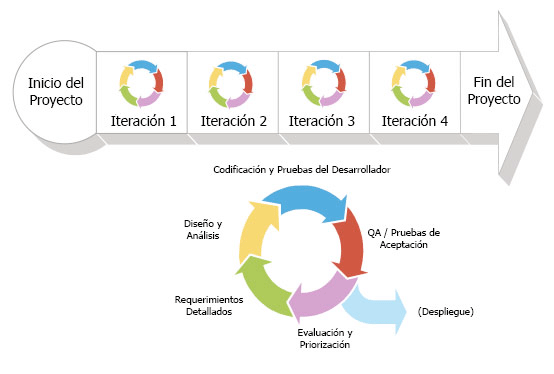
\includegraphics[width=0.8\textwidth]{../images/scrum-iteration-detail-es.png}
  \caption{Proceso de desarrollo Scrum (\url{http://www.qasoluciones.es/metodologia/agile})}
  \label{fig:diag_scrum}
  \end{center}
\end{figure}

El cambio de metodología redefine las fases en tanto en cuanto ahora debemos repetir n veces las fases de analisis, diseño, implementación, pruebas y documentación. Las horas estimadas son las mimas ya que se repartirían entre las iteraciones. De esta forma el coste del proyecto no se ve incrementado, solo la organización de las tareas y fases de cara al desarrollo del software. 

\section{Temporización}

A continuación se mostrá un diagrama de \textbf{Grantt}\footnote{Herramienta gráfica para mostrar la temporización de una serie de tareas} para ilustrar la temporización de las tareas basandonos en la planificación inicial. 

\begin{figure}[!ht]
  \begin{center}
  \includegraphics[width=0.8\textwidth]{../images/diagrama_grantt_inicial.png}
  \caption{Diagrama de Grantt inicial}
  \label{fig:diag_grant_inicial}
  \end{center}
\end{figure}

\bigskip
Aunque inicialmente se plantea una temporización basada en un número fijo de iteraciones, el proceso de desarrollo hace necesario modificar los planteamientos iniciales de horas, costes y temporización. Por ello, a continuación puede observarse una diagrama de \textbf{Grantt} con la temporización real.

\begin{figure}[!ht]
  \begin{center}
  \includegraphics[width=0.8\textwidth]{../images/diagrama_grantt_final.png}
  \caption{Diagrama de Grantt final}
  \label{fig:diag_grant_final}
  \end{center}
\end{figure}

\chapter{Análisis}

\section{Análisis de requisitos}

Todo software se desarrolla para cubrir una necesidad, por lo que en este apartado vamos a describir los requisitos que se estiman necesarios para cubrir los objetivos propuestos.

\subsection{Descripción de los actores}

Los actores implicados serán dos: el \textbf{desarrollador} y el \textbf{usuario}.

\bigskip
El \textbf{desarrollador} será el encargado de solucionar los problemas de visualización de los datos en el portal, además de portar el desarrollo actual del portal a un entorno de desarrollo continuo. También asumirá la administración del portal ya que este tipo de rol está muy integrado con las labores de despliegue en el desarrollo continuo.

\bigskip
El \textbf{usuario} de la aplicación será cualquier persona que tenga interés por conocer datos internos de la \textbf{Universidad de Granada} fácilmente. El usuario no pertenece a ningún público objetivo concreto, por lo que no se tiene que considerar que tenga una experiencia previa en navegador por sitios web.

\bigskip
Los dos tipos de actores descritos son la generalización de todo los tipos de personas que usarían el portal, sin embargo, podríamos hacer un análisis más extenso si nos basáramos en una metodología orientada al usuario como \textbf{persona}. Una persona sería la representación de usuarios que comparten objetivos y a los que se espera comportamientos similares. Un par de ejemplos:

\newpage
\begin{itemize}
	\item Alguien de la propia \textbf{Universidad de Granada} y de otra universidad que accedan al portal, ambos encajarían dentro del actor \textbf{usuario}, sin embargo eso no quiere decir que el objetivo de ambos sea el mismo, los usuarios de la propia universidad pueden querer consultar datos únicamente y los de otra universidad puede que estén más interesados en ver la estructura de las páginas del portal.
	\item Alguien que quiera hacer una despliegue de la aplicación, puede que no quiere hacerlo para una universidad sino para un ayuntamiento, volvemos a estar en el mismo caso, ambos entrarían en el tipo de actor \textbf{desarrollador}, pero sus intenciones e interés son muy distintos entre sí.
\end{itemize}

\subsection{Requisitos funcionales}

Los requisitos funcionales son las características que tiene que implementar el sistema para cubrir todas las necesidades de los distintos usuarios.

\bigskip
Al usuario lo único que le interesa es ver una página web estática con la información que desea 
consultar, para ello el desarrollador deberá hacer que sea posible que se generen siempre las tablas con los elementos de información. 

\bigskip
Por otra parte, el desarrollador quiere integrar el sistema en un desarrollo continuo, por lo que añadirá tests unitarios, test de cobertura, integración continua, despliegue automático y provisionamiento con tal fin.

\begin{itemize}
  \item \textbf{RF-1.} Administración portal:
    \begin{itemize}
    \item \textbf{RF-1.1.} Automatizar inicio del servidor del portal.
    \end{itemize}
\end{itemize}

\begin{itemize}
  \item \textbf{RF-2.} Acceso información:
    \begin{itemize}
    \item \textbf{RF-2.1.} Consultar información de \textit{Administración}.
    \item \textbf{RF-2.1.} Consultar información de \textit{Docencia}.
    \item \textbf{RF-2.1.} Consultar información de \textit{Gestión e Investigación}.
    \item \textbf{RF-2.1.} Consultar información de \textit{Normativa Legal}.
    \end{itemize}
\end{itemize}

\begin{itemize}
  \item \textbf{RF-3.} Pruebas de software:
  \begin{itemize}
    \item \textbf{RF-3.1.} Realizar tests unitarios.
    \item \textbf{RF-3.2.} Realizar test de cobertura.
    \item \textbf{RF-3.2.} Usar integración continua.
    \end{itemize}
\end{itemize}

\begin{itemize}
  \item \textbf{RF-4.} Configuración automática:
  \begin{itemize}
    \item \textbf{RF-4.1.} Usar despliegue automático.
    \item \textbf{RF-4.2.} Usar provisionamiento.
    \end{itemize}
\end{itemize}

\subsection{Requisitos no funcionales}

Los requisitos no funcionales son las características propias del desarrollo, pero que no tienen que estar relacionadas con su funcionalidad.

\begin{itemize}
  \item \textbf{RN-1.} Toda la programación del portal se hará en {\tt Node.js} y los módulos que se usen deben ser instalables a través de su gestor de paquetes {\tt NPM}.
  \item \textbf{RN-2.} El portal se iniciará y se detendrá mediante scripts lanzados con {\tt NPM}.
  \item \textbf{RN-3.} Para iniciar la ejecución del portal es necesario que reciba el puerto de escucha del servidor y la dirección de acceso.
  \item \textbf{RN-4.} Todos los módulos se ejecutarán desde scripts lanzamos con {\tt NPM}.
  \item \textbf{RN-5.} Los tests unitarios se realizarán en base a comportamientos esperados y valores de estados.
  recibidos como contestación a las peticiones que se realicen al portal.
  \item \textbf{RN-6.} Los tests unitarios tienen que recibir las páginas del portal para ejecutarse.
  \item \textbf{RN-7.} El test de cobertura tiene que tener una automatización integrable con los tests unitarios. 
  \item \textbf{RN-8.} La integración continua se ejecutará automáticamente con cada cambio que se haga en la programación del portal.
  \item \textbf{RN-9.} El despliegue automático se realizará mediante conexiones {\tt SSH}.
  \item \textbf{RN-10.} Tanto para el despliegue automático como para el provisionamiento es necesario indicar el usuario que lo realiza y el destino en el que se realiza.
\end{itemize}

\subsection{Requisitos de información}

Los requisitos de información se refieren a la información que es necesaria almacenar en el sistema. La única información relevante que se va a almacenar son los datos descriptivos y de enlace de cada uno de los elementos del portal {\tt OpenData UGR} que se van a mostrar en {\tt UGR Transparente}.

\begin{itemize}
  \item \textbf{RI-1.} Datos abiertos.
  \begin{itemize}
    \item Información sobre cada uno de los elementos que se van a mostrar en el portal de transparencia como datos abiertos.
    \item Contenido: nombre, categoría, conjunto de datos, enlace a {\tt OpenData UGR}, enlace al recurso.
  \end{itemize}
\end{itemize}

\section{Modelos de casos de uso}

Aunque ya se ha indicado que la parte funcional ya se encuentra implementada de forma previa a este proyecto, se van a incluir unos modelos de caso de uso simples para dar un visión más clara del funcionamiento general del portal {\tt UGR Transparente}.

\subsection{Descripción básica de actores}

\begin{itemize}
  \item \textbf{Ac-1.} Desarrollador.
  \begin{itemize}
   \item Descripción: Encargado del desarrollo y administración del portal.
   \item Características: Su trabajo está en el lado del servidor que genera la página, nunca trabaja desde el lado del cliente.
   \item Relaciones: Ninguna.
   \item Atributos: Ninguno.
   \item Comentarios: Es el encargado de que la información se muestre en el portal y de añadir funcionalidades al portal.
  \end{itemize}
  
  \item \textbf{Ac-2.} Usuario.
  \begin{itemize}
   \item Descripción: Persona que usa el portal para consultar datos.
   \item Características: Es el usuario común que accederá a la página.
   \item Relaciones: Ninguna.
   \item Atributos: Ninguno.
   \item Comentarios: El usuario no es necesario que tenga ningún conocimiento previo al uso del portal, simplemente accederá y consultará los datos que sean de su interés.
  \end{itemize}
\end{itemize}

\subsection{Descripción casos de uso}

\begin{itemize}
  \item \textbf{CU-1.} Inicio automático del servidor del portal.
  \begin{itemize}
    \item Actores: Desarrollador.
    \item Tipo: Primario, esencial.
    \item Referencias:
    \item Precondición: El servidor esté detenido.
    \item Postcondición: El portal será accesible públicamente.
    \item Autor: \autor.
    \item Versión: 1.0.
    \item Propósito: Iniciar el servidor del portal {\tt UGR Transparente}.
    \item Resumen: Cuando se ejecuta el script de inicio de la aplicación, arranca el servidor y el portal será accesible desde Internet.
    \begin{table}[!ht]
      \begin{center}
	\begin{tabular}{|l|l|l|l|}
	  \hline
	  \multicolumn{4}{|c|}{{\bf Curso normal}}
	  \\ \hline
	  \multicolumn{2}{|c|}{{\bf Actor}} & \multicolumn{2}{c|}{{\bf Sistema}}
	  \\ \hline
	  {\it 1} & 
	  \begin{tabular}[c]{@{}l@{}}
	    Desarrollador: da orden de\\
	    que se inicie el servidor\\
	    del portal.
	  \end{tabular} &
	  &
	  \\ \hline
	  &
	  &
	  {\it 2a} &
	  \begin{tabular}[c]{@{}l@{}}
	    Comprueba que el servidor\\
	    está detenido y lo inicia\\
	    para que el portal esté\\
	    operativo.
	  \end{tabular}
	  \\ \hline
	\end{tabular}
	\caption{Curso normal de CU-1. Inicio automático del servidor del portal}
	\label{table:cn_cu_1}
      \end{center}
    \end{table}
    \begin{table}[!ht]
      \begin{center}
	\begin{tabular}{|l|l|}
	  \hline
	  \multicolumn{2}{|c|}{{\bf Curso alterno}}
	  \\ \hline
	  {\it 2b} &
	  \begin{tabular}[c]{@{}l@{}}
	    Si el servidor está funcionando, no se ejecuta el script de\\
	    inicio del servidor.
	  \end{tabular}\\
	  \hline
	\end{tabular}
	\caption{Curso alterno de CU-1. Inicio automático del servidor del portal}
	\label{table:ca_cu_1}
      \end{center}
    \end{table}
  \end{itemize}
 
  \newpage
  \item \textbf{CU-2.} Consultar información de \textit{Administración}.
  \begin{itemize}
    \item Actores: Usuario.
    \item Tipo: Primario, esencial.
    \item Referencias:
    \item Precondición: Existan archivos con los datos abiertos.
    \item Postcondición:
    \item Autor: \autor.
    \item Versión: 1.0.
    \item Propósito: El usuario consulta datos de administración en el portal {\tt UGR Transparente}.
    \item Resumen: El usuario que accede al portal de transparencia selecciona la sección de \textit{Administración} y consulta la información de sus subsecciones.
    \begin{table}[!ht]
      \begin{center}
	\begin{tabular}{|l|l|l|l|}
	  \hline
	  \multicolumn{4}{|c|}{{\bf Curso normal}}
	  \\ \hline
	  \multicolumn{2}{|c|}{{\bf Actor}} & \multicolumn{2}{c|}{{\bf Sistema}}
	  \\ \hline
	  {\it 1} & 
	  \begin{tabular}[c]{@{}l@{}}
	    Usuario: consulta la información\\
	    de \textit{Administración} publicada en el\\
	    portal.
	  \end{tabular} &
	  &
	  \\ \hline
	  &
	  &
	  {\it 2} &
	  \begin{tabular}[c]{@{}l@{}}
	    Se generan las tablas con\\
	    todos los elementos de\\
	    información de la sección\\
	    \textit{Administración}.
	  \end{tabular}
	  \\ \hline
	  &
	  &
	  {\it 3} &
	  \begin{tabular}[c]{@{}l@{}}
	    Se muestran en la página\\
	    todos las tablas generadas\\
	    con los elementos de\\
	    información.
	  \end{tabular}
	  \\ \hline
	\end{tabular}
	\caption{Curso normal de CU-2. Consultar información de Administración}
	\label{table:cn_cu_2}
      \end{center}
    \end{table}
  \end{itemize}
  
  \newpage
  \item \textbf{CU-3.} Consultar información de \textit{Docencia}.
  \begin{itemize}
    \item Actores: Usuario.
    \item Tipo: Primario, esencial.
    \item Referencias:
    \item Precondición: Existan archivos con los datos abiertos.
    \item Postcondición:
    \item Autor: \autor.
    \item Versión: 1.0.
    \item Propósito: El usuario consulta datos de administración en el portal {\tt UGR Transparente}.
    \item Resumen: El usuario que accede al portal de transparencia selecciona la sección de \textit{Docencia} y consulta la información de sus subsecciones.
    \begin{table}[!ht]
      \begin{center}
	\begin{tabular}{|l|l|l|l|}
	  \hline
	  \multicolumn{4}{|c|}{{\bf Curso normal}}
	  \\ \hline
	  \multicolumn{2}{|c|}{{\bf Actor}} & \multicolumn{2}{c|}{{\bf Sistema}}
	  \\ \hline
	  {\it 1} & 
	  \begin{tabular}[c]{@{}l@{}}
	    Usuario: consulta la información\\
	    de \textit{Docencia} publicada en el\\
	    portal.
	  \end{tabular} &
	  &
	  \\ \hline
	  &
	  &
	  {\it 2} &
	  \begin{tabular}[c]{@{}l@{}}
	    Se generan las tablas con\\
	    todos los elementos de\\
	    información de la sección\\
	    \textit{Docencia}.
	  \end{tabular}
	  \\ \hline
	  &
	  &
	  {\it 3} &
	  \begin{tabular}[c]{@{}l@{}}
	    Se muestran en la página\\
	    todos las tablas generadas\\
	    con los elementos de\\
	    información.
	  \end{tabular}
	  \\ \hline
	\end{tabular}
	\caption{Curso normal de CU-3. Consultar información de Docencia}
	\label{table:cn_cu_3}
      \end{center}
    \end{table}
  \end{itemize}
  
  \newpage
  \item \textbf{CU-4.} Consultar información de \textit{Gestión e Investigación}.
  \begin{itemize}
    \item Actores: Usuario.
    \item Tipo: Primario, esencial.
    \item Referencias:
    \item Precondición: Existan archivos con los datos abiertos.
    \item Postcondición:
    \item Autor: \autor.
    \item Versión: 1.0.
    \item Propósito: El usuario consulta datos de administración en el portal {\tt UGR Transparente}.
    \item Resumen: El usuario que accede al portal de transparencia selecciona la sección de \textit{Gestión e Investigación} y consulta la información de sus subsecciones.
    \begin{table}[!ht]
      \begin{center}
	\begin{tabular}{|l|l|l|l|}
	  \hline
	  \multicolumn{4}{|c|}{{\bf Curso normal}}
	  \\ \hline
	  \multicolumn{2}{|c|}{{\bf Actor}} & \multicolumn{2}{c|}{{\bf Sistema}}
	  \\ \hline
	  {\it 1} & 
	  \begin{tabular}[c]{@{}l@{}}
	    Usuario: consulta la información\\
	    de \textit{Gestión e Investigación} publicada\\
	    en el portal.
	  \end{tabular} &
	  &
	  \\ \hline
	  &
	  &
	  {\it 2} &
	  \begin{tabular}[c]{@{}l@{}}
	    Se generan las tablas con\\
	    todos los elementos de\\
	    información de la sección\\
	    \textit{Gestión e Investigación}.
	  \end{tabular}
	  \\ \hline
	  &
	  &
	  {\it 3} &
	  \begin{tabular}[c]{@{}l@{}}
	    Se muestran en la página\\
	    todos las tablas generadas\\
	    con los elementos de\\
	    información.
	  \end{tabular}
	  \\ \hline
	\end{tabular}
	\caption{Curso normal de CU-4. Consultar información de Gestión e Investigación}
	\label{table:cn_cu_4}
      \end{center}
    \end{table}
  \end{itemize}
  
  \newpage
  \item \textbf{CU-5.} Consultar información de \textit{Normativa Legal}.
  \begin{itemize}
    \item Actores: Usuario.
    \item Tipo: Primario, esencial.
    \item Referencias:
    \item Precondición: Existan archivos con los datos abiertos.
    \item Postcondición:
    \item Autor: \autor.
    \item Versión: 1.0.
    \item Propósito: El usuario consulta datos de administración en el portal {\tt UGR Transparente}.
    \item Resumen: El usuario que accede al portal de transparencia selecciona la sección de \textit{Normativa Legal} y consulta la información de sus subsecciones.
    \begin{table}[!ht]
      \begin{center}
	\begin{tabular}{|l|l|l|l|}
	  \hline
	  \multicolumn{4}{|c|}{{\bf Curso normal}}
	  \\ \hline
	  \multicolumn{2}{|c|}{{\bf Actor}} & \multicolumn{2}{c|}{{\bf Sistema}}
	  \\ \hline
	  {\it 1} & 
	  \begin{tabular}[c]{@{}l@{}}
	    Usuario: consulta la información\\
	    de \textit{Normativa Legal} publicada en el\\
	    portal.
	  \end{tabular} &
	  &
	  \\ \hline
	  &
	  &
	  {\it 2} &
	  \begin{tabular}[c]{@{}l@{}}
	    Se generan las tablas con\\
	    todos los elementos de\\
	    información de la sección\\
	    \textit{Normativa Legal}.
	  \end{tabular}
	  \\ \hline
	  &
	  &
	  {\it 3} &
	  \begin{tabular}[c]{@{}l@{}}
	    Se muestran en la página\\
	    todos las tablas generadas\\
	    con los elementos de\\
	    información.
	  \end{tabular}
	  \\ \hline
	\end{tabular}
	\caption{Curso normal de CU-5. Consultar información de Normativa Legal}
	\label{table:cn_cu_5}
      \end{center}
    \end{table}
  \end{itemize}
 
  \newpage
  \item \textbf{CU-6.} Realizar tests unitarios.
  \begin{itemize}
    \item Actores: Desarrollador.
    \item Tipo: Primario, esencial.
    \item Referencias:
    \item Precondición: Existan tests unitarios.
    \item Postcondición: 
    \item Autor: \autor.
    \item Versión: 1.0.
    \item Propósito: Realizar tests unitarios para comprobar las funcionalidades de la aplicación.
    \item Resumen: Cada vez que se añadan nuevas páginas o funcionalidades al portal, se comprueba que funcionan correctamente.
    \begin{table}[!ht]
      \begin{center}
	\begin{tabular}{|l|l|l|l|}
	  \hline
	  \multicolumn{4}{|c|}{{\bf Curso normal}}
	  \\ \hline
	  \multicolumn{2}{|c|}{{\bf Actor}} & \multicolumn{2}{c|}{{\bf Sistema}}
	  \\ \hline
	  {\it 1} & 
	  \begin{tabular}[c]{@{}l@{}}
	    Desarrollador: da orden de\\
	    ejecutar los tests unitarios.
	  \end{tabular} &
	  &
	  \\ \hline
	  &
	  &
	  {\it 2a} &
	  \begin{tabular}[c]{@{}l@{}}
	    Comprueba que hay tests\\
	    unitarios y los ejecuta.\\
	  \end{tabular}
	  \\ \hline
	\end{tabular}
	\caption{Curso normal de CU-6. Realizar tests unitarios}
	\label{table:cn_cu_6}
      \end{center}
    \end{table}
    \begin{table}[!ht]
      \begin{center}
	\begin{tabular}{|l|l|}
	  \hline
	  \multicolumn{2}{|c|}{{\bf Curso alterno}}
	  \\ \hline
	  {\it 2b} &
	  \begin{tabular}[c]{@{}l@{}}
	    Si no hay tests unitarios creados, el sistema no hace nada.
	  \end{tabular}\\
	  \hline
	\end{tabular}
	\caption{Curso alterno de CU-6. Realizar tests unitarios}
	\label{table:ca_cu_6}
      \end{center}
    \end{table}
  \end{itemize}
 
  \newpage
  \item \textbf{CU-7.} Realizar tests de cobertura.
  \begin{itemize}
    \item Actores: Desarrollador.
    \item Tipo: Primario, esencial.
    \item Referencias: (CU-6.) Realizar tests unitarios.
    \item Precondición: Existan tests unitarios.
    \item Postcondición: 
    \item Autor: \autor.
    \item Versión: 1.0.
    \item Propósito: Realizar test de cobertura para comprobar calidad de los tests unitarios.
    \item Resumen: Para comprobar si los tests unitarios cumplen correctamente con su función se analiza el porcentaje del código que está cubierto por los mismos.
    \begin{table}[!ht]
      \begin{center}
	\begin{tabular}{|l|l|l|l|}
	  \hline
	  \multicolumn{4}{|c|}{{\bf Curso normal}}
	  \\ \hline
	  \multicolumn{2}{|c|}{{\bf Actor}} & \multicolumn{2}{c|}{{\bf Sistema}}
	  \\ \hline
	  {\it 1} & 
	  \begin{tabular}[c]{@{}l@{}}
	    Desarrollador: da orden de\\
	    ejecutar test de cobertura.
	  \end{tabular} &
	  &
	  \\ \hline
	  &
	  &
	  {\it 2a} &
	  \begin{tabular}[c]{@{}l@{}}
	    Comprueba que hay tests\\
	    unitarios y los ejecuta.\\
	  \end{tabular}
	  \\ \hline
	  &
	  &
	  {\it 3} &
	  \begin{tabular}[c]{@{}l@{}}
	    Se ejecuta el test de \\
	    cobertura en base a los\\
	    tests unitarios ejecutados.
	  \end{tabular}
	  \\ \hline
	\end{tabular}
	\caption{Curso normal de CU-7. Realizar test de cobertura}
	\label{table:cn_cu_7}
      \end{center}
    \end{table}
    \begin{table}[!ht]
      \begin{center}
	\begin{tabular}{|l|l|}
	  \hline
	  \multicolumn{2}{|c|}{{\bf Curso alterno}}
	  \\ \hline
	  {\it 2b} &
	  \begin{tabular}[c]{@{}l@{}}
	    Si no hay tests unitarios creados, el sistema no hace nada.
	  \end{tabular}\\
	  \hline
	\end{tabular}
	\caption{Curso alterno de CU-7. Realizar test de cobertura}
	\label{table:ca_cu_7}
      \end{center}
    \end{table}
  \end{itemize}
 
  \newpage
  \item \textbf{CU-8.} Usar integración continua.
  \begin{itemize}
    \item Actores: Desarrollador.
    \item Tipo: Primario, esencial.
    \item Referencias: (CU-5.) Realizar tests unitarios.
    \item Precondición: Existan test unitarios.
    \item Postcondición: Se genera un informe con el resultado de los tests unitarios.
    \item Autor: \autor.
    \item Versión: 1.0.
    \item Propósito: Comprobar si los cambios en la aplicación provocan errores.
    \item Resumen: Cuando se efectúan cambios en la aplicación automáticamente se ejecutan los tests unitarios para comprobar si los cambios introducidos provocan conflictos en la plataforma.
    \begin{table}[!ht]
      \begin{center}
	\begin{tabular}{|l|l|l|l|}
	  \hline
	  \multicolumn{4}{|c|}{{\bf Curso normal}}
	  \\ \hline
	  \multicolumn{2}{|c|}{{\bf Actor}} & \multicolumn{2}{c|}{{\bf Sistema}}
	  \\ \hline
	  {\it 1} & 
	  \begin{tabular}[c]{@{}l@{}}
	    Desarrollador: guardar\\
	    cambios en el repositorio.
	  \end{tabular} &
	  &
	  \\ \hline
	  &
	  &
	  {\it 2a} &
	  \begin{tabular}[c]{@{}l@{}}
	    Comprueba que hay tests\\
	    unitarios y comienza la\\
	    verificación de la\\
	    integración continua.
	  \end{tabular}
	  \\ \hline
	  &
	  &
	  {\it 3} &
	  \begin{tabular}[c]{@{}l@{}}
	    Ejecuta los tests unitarios\\
	    para cada entorno definido.
	  \end{tabular}
	  \\ \hline
	\end{tabular}
	\caption{Curso normal de CU-8. Usar integración continua}
	\label{table:cn_cu_8}
      \end{center}
    \end{table}
    \begin{table}[!ht]
      \begin{center}
	\begin{tabular}{|l|l|}
	  \hline
	  \multicolumn{2}{|c|}{{\bf Curso alterno}}
	  \\ \hline
	  {\it 2b} &
	  \begin{tabular}[c]{@{}l@{}}
	    Si no hay tests unitarios creados, el sistema no hace nada.
	  \end{tabular}\\
	  \hline
	\end{tabular}
	\caption{Curso alterno de CU-8. Usar integración continua}
	\label{table:ca_cu_8}
      \end{center}
    \end{table}
  \end{itemize}
 
  \newpage
  \item \textbf{CU-.9 } Usar despliegue automático.
  \begin{itemize}
    \item Actores: Desarrollador.
    \item Tipo: Primario, esencial.
    \item Referencias: (CU-1.) Iniciar plataforma.
    \item Precondición: 
    \item Postcondición: Los cambios introducidos son aplicados en la plataforma.
    \item Autor: \autor.
    \item Versión: 1.0.
    \item Propósito: Aplicar automáticamente los cambios realizados a la aplicación. 
    \item Resumen: Para no tener que acceder manualmente al servidor de la plataforma y tener que desplegar los cambios introducidos, desde el entorno de desarrollo desplegamos automáticamente los cambios en el servidor.
    \begin{table}[!ht]
      \begin{center}
	\begin{tabular}{|l|l|l|l|}
	  \hline
	  \multicolumn{4}{|c|}{{\bf Curso normal}}
	  \\ \hline
	  \multicolumn{2}{|c|}{{\bf Actor}} & \multicolumn{2}{c|}{{\bf Sistema}}
	  \\ \hline
	  {\it 1} & 
	  \begin{tabular}[c]{@{}l@{}}
	    Desarrollador: ordenar\\
	    despliegue automático.
	  \end{tabular} &
	  &
	  \\ \hline
	  &
	  &
	  {\it 2} &
	  \begin{tabular}[c]{@{}l@{}}
	    Conectar al servidor.
	  \end{tabular}
	  \\ \hline
	  &
	  &
	  {\it 3} &
	  \begin{tabular}[c]{@{}l@{}}
	    Crear copia de seguridad.
	  \end{tabular}
	  \\ \hline
	  &
	  &
	  {\it 4a} &
	  \begin{tabular}[c]{@{}l@{}}
	    Comprobar si hay cambios en\\
	    el repositorio de la\\
	    plataforma y descargarlos\\
	    en dicho caso.
	  \end{tabular}
	  \\ \hline
	  &
	  &
	  {\it 5} &
	  \begin{tabular}[c]{@{}l@{}}
	    Iniciar la plataforma con\\
	    los cambios aplicados.
	  \end{tabular}
	  \\ \hline
	\end{tabular}
	\caption{Curso normal de CU-9. Usar despliegue automático}
	\label{table:cn_cu_9}
      \end{center}
    \end{table}
    \begin{table}[!ht]
      \begin{center}
	\begin{tabular}{|l|l|}
	  \hline
	  \multicolumn{2}{|c|}{{\bf Curso alterno}}
	  \\ \hline
	  {\it 4b} &
	  \begin{tabular}[c]{@{}l@{}}
	    Si no hay cambios aplicables, se continua con el proceso.
	  \end{tabular}\\
	  \hline
	\end{tabular}
	\caption{Curso alterno de CU-9. Usar despliegue automático}
	\label{table:ca_cu_9}
      \end{center}
    \end{table}
  \end{itemize}
 
  \newpage
  \item \textbf{CU-.10} Usar provisionamiento.
  \begin{itemize}
    \item Actores: Desarrollador.
    \item Tipo: Primario, esencial.
    \item Referencias: (CU-1.) Iniciar plataforma.
    \item Precondición: 
    \item Postcondición: El portal queda instalado en la infraestructura seleccionada.
    \item Autor: \autor.
    \item Versión: 1.0.
    \item Propósito: Instalar automáticamente el portal en una infraestructura dada.
    \item Resumen: Se instalarán automáticamente todos los elementos necesarios para poner en funcionamiento el portal en cualquier infraestructura que se indique.
    \begin{table}[!ht]
      \begin{center}
	\begin{tabular}{|l|l|l|l|}
	  \hline
	  \multicolumn{4}{|c|}{{\bf Curso normal}}
	  \\ \hline
	  \multicolumn{2}{|c|}{{\bf Actor}} & \multicolumn{2}{c|}{{\bf Sistema}}
	  \\ \hline
	  {\it 1} & 
	  \begin{tabular}[c]{@{}l@{}}
	    Desarrollador: ordenar\\
	    despliegue automático.
	  \end{tabular} &
	  &
	  \\ \hline
	  &
	  &
	  {\it 2} &
	  \begin{tabular}[c]{@{}l@{}}
	    Conectar al servidor.
	  \end{tabular}
	  \\ \hline
	  &
	  &
	  {\it 3} &
	  \begin{tabular}[c]{@{}l@{}}
	    Comprobar aplicación necesaria.
	  \end{tabular}
	  \\ \hline
	  &
	  &
	  {\it 4a} &
	  \begin{tabular}[c]{@{}l@{}}
	    Se comprueba si la aplicación\\
	    necesaria está instalada,\\
	    instalándola en caso de que\\
	    no lo esté.
	  \end{tabular}
	  \\ \hline
	  &
	  &
	  {\it 5} &
	  \begin{tabular}[c]{@{}l@{}}
	    Descarga la plataforma desde\\
	    el repositorio.
	  \end{tabular}
	  \\ \hline
	  &
	  &
	  {\it 6} &
	  \begin{tabular}[c]{@{}l@{}}
	    Instalar todas las dependencias\\
	    de la plataforma.
	  \end{tabular}
	  \\ \hline
	  &
	  &
	  {\it 7} &
	  \begin{tabular}[c]{@{}l@{}}
	    Se establecen los parámetros de\\
	    acceso al portal desde Internet.
	  \end{tabular}
	  \\ \hline
	  &
	  &
	  {\it 8} &
	  \begin{tabular}[c]{@{}l@{}}
	    Con todo preparado, se inicia\\
	    la plataforma.
	  \end{tabular}
	  \\ \hline
	\end{tabular}
	\caption{Curso normal de CU-10. Usar provisionamiento}
	\label{table:cn_cu_10}
      \end{center}
    \end{table}
    \begin{table}[!ht]
      \begin{center}
	\begin{tabular}{|l|l|}
	  \hline
	  \multicolumn{2}{|c|}{{\bf Curso alterno}}
	  \\ \hline
	  {\it 4b} &
	  \begin{tabular}[c]{@{}l@{}}
	    Si la aplicación está instalada, se continua con el proceso.
	  \end{tabular}\\
	  \hline
	\end{tabular}
	\caption{Curso alterno de CU-10. Usar provisionamiento}
	\label{table:ca_cu_10}
      \end{center}
    \end{table}
  \end{itemize}
 \end{itemize}

\newpage
\section{Diagrama de paquetes}

Este diagrama representa la estructura lógica del sistema basado en las dependencias existentes entre sí. El paquete de \textbf{Configuración automática} depende del paquete \textbf{Administración portal} porque necesita de tareas de administración como es iniciar el servidor.

\begin{figure}[!ht]
  \begin{center}
  \includegraphics[width=0.8\textwidth]{../images/diagrama_paquetes.png}
  \caption{Diagrama de paquetes}
  \label{fig:diag_paquetes}
  \end{center}
\end{figure}
 
\section{Diagramas de casos de uso}

Los diagramas de casos de uso representa como los diferentes actores se relacionan con el sistema para usar sus funciones. Por ejemplo, en el primer caso de uso vemos como el \textbf{desarrollador} se relaciona con el sistema para iniciar el servidor del portal, mientras, en el segundo vemos como el \textbf{usuario} se relaciona con el sistema para consultar la información de las diferentes secciones del portal.

\begin{figure}[!ht]
  \begin{center}
  \includegraphics[width=0.65\textwidth]{../images/diag_cu_ap.png}
  \caption{Diagrama de casos de uso: paquete Administración portal}
  \label{fig:diag_cu_ap}
  \end{center}
\end{figure}

\begin{figure}[!ht]
  \begin{center}
  \includegraphics[width=0.65\textwidth]{../images/diag_cu_ai.png}
  \caption{Diagrama de casos de uso: paquete Acceso información}
  \label{fig:diag_cu_ai}
  \end{center}
\end{figure}

\newpage
\
\newpage
En el tercer diagrama vemos como el \textbf{desarrollador} se relaciona con los procesos relacionadas con las pruebas (que a su vez son dependientes entre sí); y en el cuarto vemos como también el \textbf{desarrollador} se relaciona con el sistema para realizar las tareas de configuración automática, como son el despliegue automático y el provisionamiento.

\begin{figure}[!ht]
  \begin{center}
  \includegraphics[width=0.65\textwidth]{../images/diag_cu_ps.png}
  \caption{Diagrama de casos de uso: paquete Pruebas de software}
  \label{fig:diag_cu_ps}
  \end{center}
\end{figure}

\begin{figure}[!ht]
  \begin{center}
  \includegraphics[width=0.65\textwidth]{../images/diag_cu_ca.png}
  \caption{Diagrama de casos de uso: paquete Configuración automática}
  \label{fig:diag_cu_ca}
  \end{center}
\end{figure}

\newpage
\section{Diagramas de actividad}

Los diagramas de actividad sirven para representar la descomposición de un proceso en las diferentes acciones de las que está compuesto. Las actividades de consultar algún tipo de información son procedimiento secuenciales en los que la ejecución es bastante simple; pero la actividad de iniciar el servidor del portal, realizar los test unitarios, realizar los test de cobertura, usar la integración continua tienen situaciones condicionales que son los que dan lugar a cursos alternos de la ejecución. Las actividades de despliegue automático y provisionamiento además tienen también puntos de sincronización que harán que el proceso siga el mismo cauce en su ejecución.

\begin{figure}[!ht]
  \begin{center}
  \includegraphics[width=1\textwidth]{../images/diag_act_cu_01.png}
  \caption{Diagrama de actividad CU-1. Inicio automático del servidor del portal}
  \label{fig:diag_act_cu_01}
  \end{center}
\end{figure}

\begin{figure}[!ht]
  \begin{center}
  \includegraphics[width=1\textwidth]{../images/diag_act_cu_02.png}
  \caption{Diagrama de actividad CU-2. Consultar información de Administración}
  \label{fig:diag_act_cu_02}
  \end{center}
\end{figure}

\begin{figure}[!ht]
  \begin{center}
  \includegraphics[width=1\textwidth]{../images/diag_act_cu_03.png}
  \caption{Diagrama de actividad CU-3. Consultar información de Docencia}
  \label{fig:diag_act_cu_03}
  \end{center}
\end{figure}

\begin{figure}[!ht]
  \begin{center}
  \includegraphics[width=1\textwidth]{../images/diag_act_cu_04.png}
  \caption{Diagrama de actividad CU-4. Consultar información de Gestión e Investigación}
  \label{fig:diag_act_cu_04}
  \end{center}
\end{figure}

\begin{figure}[!ht]
  \begin{center}
  \includegraphics[width=1\textwidth]{../images/diag_act_cu_05.png}
  \caption{Diagrama de actividad CU-5. Consultar información de Normativa Legal}
  \label{fig:diag_act_cu_05}
  \end{center}
\end{figure}

\begin{figure}[!ht]
  \begin{center}
  \includegraphics[width=1\textwidth]{../images/diag_act_cu_06.png}
  \caption{Diagrama de actividad CU-6. Realizar tests unitarios}
  \label{fig:diag_act_cu_06}
  \end{center}
\end{figure}

\begin{figure}[!ht]
  \begin{center}
  \includegraphics[width=1\textwidth]{../images/diag_act_cu_07.png}
  \caption{Diagrama de actividad CU-7. Realizar test de cobertura}
  \label{fig:diag_act_cu_07}
  \end{center}
\end{figure}

\begin{figure}[!ht]
  \begin{center}
  \includegraphics[width=1\textwidth]{../images/diag_act_cu_08.png}
  \caption{Diagrama de actividad CU-8. Usar integración continua}
  \label{fig:diag_act_cu_08}
  \end{center}
\end{figure}

\begin{figure}[!ht]
  \begin{center}
  \includegraphics[width=1\textwidth]{../images/diag_act_cu_09.png}
  \caption{Diagrama de actividad CU-9. Usar despliegue automático}
  \label{fig:diag_act_cu_09}
  \end{center}
\end{figure}

\begin{figure}[!ht]
  \begin{center}
  \includegraphics[width=1\textwidth]{../images/diag_act_cu_10.png}
  \caption{Diagrama de actividad CU-10. Usar provisionamiento}
  \label{fig:diag_act_cu_10}
  \end{center}
\end{figure}

\newpage
\
\newpage
\
\newpage
\
\newpage
\
\newpage
\
\newpage
\
\newpage
\
\newpage
\
\newpage

\section{Diagrama conceptual}

En el diagrama conceptual podemos ver una representación de la estructura de la implementación. A excepción de la clase \textbf{test}, todas las clases son parte de la aplicación principal (\textbf{app}) por lo que tienen una relación de composición con la misma y no tienen sentido sin esta. Las clases de \textbf{test} y \textbf{app} tiene una relación de agrupación, porque el módulo test puede realizar las pruebas sobre cualquier módulo de aplicación que sea recibido.

\begin{figure}[!ht]
  \begin{center}
  \includegraphics[width=1\textwidth]{../images/diagrama_conceptual.png}
  \caption{Diagrama conceptual}
  \label{fig:diagrama_conceptual}
  \end{center}
\end{figure}

\section{Otros diagramas o interfaces}

Gran parte de la implementación no va a ser de la aplicación principal en si misma, sino herramientas que se le van a agregar para obtener diferentes funcionalidades que se usarán durante su desarrollo, de ahí que no se considere necesario el realizar diagramas de comunicación ni diagramas de secuencia.

\bigskip
En cuanto a la interfaz gráfica, no será necesaria porque todas las herramientas solo tienen modo de funcionamiento a través de terminal.
\chapter{Diseño}

\section{Diseño general del portal}

Para describir el diseño que se va a seguir en la programación del proyecto hay que tener en cuenta que se va a usar {\tt Node.js}, que está basado en el lenguaje de programación {\tt JavaScript} (que es un lenguaje orientado a objetos). Se usará un paradigma de programación orientado a objetos con diversas clases, que en este entorno de programación suelen ser referidos como módulos.

\bigskip
Existirá un módulo principal de la plataforma ({\tt app.js}) que será la plataforma en si misma, que es el encargado de generar el servidor al que se realizarán las peticiones y visualizar cada unas de las páginas. Existirán también un módulo por cada una de las secciones del portal: \textit{Administración} ({\tt administración.js}), \textit{Docencia} ({\tt docencia.js}), \textit{Gestión e Investigación} ({\tt gestionInvestigacion.js}) y \textit{Normativa Legal} ({\tt normativaLegal.js}. Si comparamos este esquema con el de una aplicación más tradicional, podríamos considerar el módulo ({\tt app.js}) como la clase principal y el resto de módulos como otras clases que tienen como función ser atributos compuestos de esa clase principal.

\bigskip
Cada uno de estos módulos de las diversas secciones, obtendrá la información para generar las páginas de sus subsecciones desde un archivo de datos \textit{JSON}, organizados de la siguiente forma.

\newpage
\begin{itemize}
 \item {\tt UGR Transparente} ({\tt app.js}).
 \begin{itemize}
  \item \textit{Administración} ({\tt administración.js}).
  \begin{itemize}
   \item \textit{Personal} ({\tt personal.json}).
   \item \textit{Información Económica} ({\tt infoEcononica.json}).
   \item \textit{Servicios} ({\tt servicios.json}).
  \end{itemize}
  \item \textit{Docencia}.
  \begin{itemize}
   \item \textit{Oferta y Demanda Académica} ({\tt ofertaDemanda.json}).
   \item \textit{Claustro} ({\tt claustro.json}).
   \item \textit{Estudiantes} ({\tt estudiantes.json}).
  \end{itemize}
  \item \textit{Gestión e Investigación}.
  \begin{itemize}
   \item \textit{Misión} ({\tt mision.json}).
   \item \textit{Plan Estratégico} ({\tt .json}).
   \item \textit{Gobierno} ({\tt gobierno.json}).
   \item \textit{Estadísticas} ({\tt estadistica.json}).
  \end{itemize}
  \item \textit{Normativa Legal}.
  \begin{itemize}
   \item \textit{Normativa Legal} ({\tt normativaLegal.json}).
  \end{itemize}
 \end{itemize}
\end{itemize}

Cada vez que un usuario quiere consultar la información de una subsección, el portal de transparencia ({\tt UGR Transparente}) hace una llamada al método de generación de la página de la sección elegida para su subsección determinada; ese método, procesará la plantilla {\tt Jade} para la página pasándole el archivo \textit{JSON} de datos y el resultado final será la página web que será visible en el portal.

\bigskip
De igual forma a lo mencionado de la aplicación del portal de transparencia, los test unitarios ({\tt test.js}) y el despliegue automático ({\tt flightplan.js}) son otros módulos que ejecutan dichas acciones, el test de cobertura se realiza automáticamente a partir de los test unitarios, la integración continua se realiza en base a la configuración del archivo {\tt .travis.yml}, y finalmente, el provisionamiento sigue las tareas en el archivo de configuración {\tt transparente.yml}. Todos estos módulos son independientes del funcionamiento del módulo principal, y simplemente llamaremos cuando queramos hacer uso de sus funcionalidades.

\newpage
\section{Diseño de una aplicación con desarrollo colaborativo}

En varias ocasiones se ha indicado que este proyecto parte de un desarrollo colaborativo, esto es debido a que hoy en día es muy difícil concebir un proyecto de software libre fuera de un entorno colaborativo que permita publicar el código libremente en Internet donde sea accesible por cualquier persona, esta filosofía es la que sigue por ejemplo el desarrollo de {\tt Linux} a principio de los años 90, el que se podría considerar como el más grande y relevante proyecto de software libre a nivel mundial. Además de abogar por la transparencia, este sistema de desarrollo hace que se más fácil encontrar errores durante el desarrollo ya que un mayor número de personas tienen acceso total al mismo. También hay que tener en cuenta como en todo proyecto que es imprescindible una herramienta de control de versiones, aún más en uno colaborativo donde es fácil que se produzcan conflictos en los archivos modificados por unos y otros desarrolladores.

\bigskip
La plataforma de desarrollo colaborativo y la herramienta de control de versiones a usar son {\tt GitHub} y {\tt Git} respectivamente. {\tt GitHub} es una de las plataformas de desarrollo colaborativo más usadas en proyectos libres y usa {\tt Git} como sistema de control de versiones para gestionar los proyectos que se almacenan en la plataforma. Estás son las herramientas que nos van a permitir que nuestro proyecto se convierta en un proyecto que se desarrollo de forma ágil, concretamente se va a seguir una metodología \textit{DevOps}.

\bigskip
Una metodología de desarrollo \textit{DevOps} consiste inicialmente en no hacer distinción entre el desarrollo del software y la administración del mismo, todo estará comunicado para que sea posible realizar entregas del software de forma frecuente asegurándose de que esas mismas entregas continuas no sea el origen de fallos futuros. La forma de asegurarse de que esos fallos no se producirán es dividir todo el desarrollo en fases que tengan que realizarse secuencialmente, controlando a cada fase que no se produzcan errores en la misma; como una cadena de montaje en la que podemos estar seguro de que el producto que llega al final está en perfectas condiciones, porque en caso contrario hubiera sido retirado durante el proceso.

\bigskip
En este proyecto, hemos considerado que las fases que nos permitirían asegurarnos que el producto que sale de la cadena de montaje en perfectas condiciones sean los test unitarios, la integración continua y el despliegue automático, todo esto apoyado en un sistema de control de versiones y una plataforma de desarrollo colaborativo abierto. Además, también se usará provisionamiento para facilitar la portabilidad del portal de una infraestructura a otra distinta. 

\section{Diseño de los tests unitarios y test de cobertura}

Para cumplir la parte de testeo de la implementación de la metodología \textit{DevOps}, a partir del desarrollo de este proyecto se pretende seguir un desarrollo guiado por pruebas (en inglés, \textit{Test-Driven Development} o \textit{TDD}). Esto consiste en escribir primero las pruebas que consideremos que la aplicación debe superar y luego desarrollar el código que realice la función que queremos cumplir, pero superando dichas pruebas. 

\bigskip
Estas pruebas estarán basadas en la ejecución de tests unitarios que estarán diseñados para comprobar de forma de automática que el código escrito cumple con el objetivo determinado; por lo que si una vez ejecutamos todos los tests unitarios no obtenemos que todos han tenido una ejecución exitosa, tenemos que revisar el código escrito para saber por qué fallan.

\bigskip
Haciendo esto nos aseguraremos que todos las funcionalidades que vayamos añadiendo a la implementación de la aplicación funcionarán correctamente; también nos asegura que si tenemos que hacer grandes modificaciones en el código, siempre que estas modificaciones sigan pasando las pruebas, no deberemos preocuparnos por estropear el funcionamiento de la aplicación.

\bigskip
El tipo de test unitario que vamos a usar es un test basado en el comportamiento, es decir, la forma de evaluar si un test se supera con éxito o fracaso es mediante la comprobación de la respuesta que da nuestra aplicación ante una solicitud 
determinada. Ejemplos:

\begin{itemize}
 \item Para comprobar que un archivo con datos de configuración ha sido cargado, el archivo cargado no debe ser nulo.
 \item Para comprobar que en la información cargado se encuentra el nombre de la categoría, la categoría debe tener una propiedad llamada ``nombre''.
 \item Para comprobar que las páginas del portal están accesibles, las respuesta a las solicitudes se espera que tenga el valor 200 (código de respuesta estándar para peticiones correctas en conexiones \textit{HTTP}).
\end{itemize}

Pero el diseño de las pruebas no termina con escribir los tests unitarios que consideremos oportunos, también es necesario que esos tests pasen a su vez un test de cobertura. Un test de cobertura comprueba el porcentaje de código desarrollado y/o número de funciones de la aplicación que se están evaluando con los tests unitarios desarrollados, con esto se puede verificar la completitud de los tests unitarios; si todos nuestros tests unitarios se evalúan correctamente, pero solo están cubriendo un 30\% del total de la aplicación, este resultado satisfactorio no nos puede asegurar que la funcionalidad completa de la aplicación se vaya a ejecutar sin problemas.

\bigskip
Los tests unitarios se van a desarrollar usando {\tt Should} y {\tt Supertest}, ambos módulos de {\tt Node.js} para evaluar comportamientos en las peticiones. Estos tests unitarios a su vez van a ser evaluados por {\tt Mocha}, un framework de {\tt JavaScript} para testeo que se ejecuta tanto en aplicaciones {\tt Node.js} como en navegadores web. Por último, todo esto pasará por las pruebas de cobertura de código de {\tt Istanbul}, que generará un informa detallado especificando la cantidad de código y el número de funciones que están cubiertas y también los que no.

\section{Diseño de la integración continua}

La integración continua (en inglés, \textit{continuous integration} o \textit{CI}) consiste en comprobar cada vez que hacemos cambios en el código de la aplicación esto no genere problemas en su ejecución, ya que el cambio del comportamiento en una simple función puede cambiar en gran parte el comportamiento de la aplicación entera, y si otra función requiere del resultado de esta última, las consecuencias pueden ser desastrosas. Teniendo en cuenta que vamos a trabajar en un entorno de desarrollo colaborativo, es todavía más necesario que se asegure la integridad de la aplicación frente a los cambios.

\bigskip
Para que esto se pueda realizar, con cada cambios se activará automáticamente un proceso que verificará mediante la ejecución de los tests unitarios escritos que los cambios realizados no producen errores en la aplicación. Al igual que pasaba con los tests unitarios, la integración continua es una medida que nos permite incrementar la calidad del software producido porque cuanto más a menudo se hagan estas comprobaciones, mayor será la facilidad para detectar fallos en el propio software.

\bigskip
Realizaremos la integración continua a través de {\tt Travis CI}, que es un sistema distribuido de integración continua libre que está integrado con {\tt GitHub}. Este sistema además tiene como ventajas el soporte para numerosos lenguajes y la posibilidad de ejecutar las pruebas en distintas versiones del propio lenguaje, por lo que fácilmente podríamos probar nuestro desarrollo con diferentes configuraciones sin tener que realizar cambios en nuestro sistema local.

\bigskip
El procedimiento para realizar la integración continua consistirá en configurar el repositorio del proyecto en {\tt GitHub} para que cada vez se realice un cambio en los archivos del repositorio, este iniciará un proceso por el cual se creará un \textit{build} automático en un servidor virtual de {\tt Travis CI} que se ha creado con tal finalidad y se desplegará en él la última versión con los cambios que acabamos de realizar, para acto seguido ejecutar las pruebas que hayamos desarrollado y generar un informe sobre los resultados de las pruebas para cada una de las configuraciones que hayamos definido para la integración continua. Estos informes son almacenados en el propio sitio de {\tt Travis}, recibiendo un aviso por correo en el caso de que las pruebas no hayan finalizado exitosamente en alguna de las configuraciones.

\section{Diseño del despliegue automático}

Una vez que tenemos la seguridad de que toda la aplicación funciona correctamente, solo nos queda desplegarla en nuestro servidor de producción; además, vamos a automatizar las tareas que deberíamos realizar manualmente para evitar posibles errores. En esto consiste el despliegue automático, hacer efectivos los cambios en nuestro software de nuestro software en una o varias plataformas objetivo sin que tengamos que realizar personalmente y paso a paso el proceso necesario para ello, todo es 
automatizado.

\bigskip
Antes de pasar a implementar el despliegue automático, hay que pensar que tareas es necesario o queremos que se realicen. Independientemente del tipo de aplicación, como medida preventiva se debe hacer una copia de seguridad del estado actual de la aplicación desplegada en el servidor. La ejecución del portal depende de que el servidor creado por {\tt Express} esté en ejecución, por lo que antes de desplegar la nueva versión, se debería detener la ejecución de la versión anterior. Con todo esto hecho solo nos quedaría obtener los propios cambios realizamos, comprobar que todas las dependencias se siguen cumpliendo y establecer los parámetros para que el servidor sea accesible desde Internet; para finalizar la tarea, se iniciaría la ejecución de la aplicación.

\bigskip
Todas las tareas descritas, queremos que sean ejecutadas de forma secuencial una tras otra, de forma automática y necesitar la interacción con el usuario. Para cumplir esto usaremos {\tt Flightplan}, un módulo de {\tt Node.js} que nos permite coordinar de forma automática el despliegue de aplicaciones con tareas de administración del sistema.

\newpage
\section{Diseño del provisionamiento}

Con toda la aplicación ya realizada, para su instalación inicial en un plataforma determinada primero tenemos que provisionarla con todos los recursos software necesarios. Encontraremos una mayor cantidad de referencias a este procedimiento por su término en ingles, \textit{software provisioning}, ya que el termino en español es una traducción literal que salvo por el acompañamiento del termino \textit{``software''}, puede referirse a abastecimientos de recursos necesarios en general no necesariamente relacionado con el campo de la informática.

\bigskip
Entre el software básico necesario hay que considerar para instalar la propia plataforma del desarrollo de la aplicación ({\tt Node.js}) y la herramienta de control de versiones ({\tt Git}). Con esto instalado, se clona el repositorio en {\tt GitHub} del proyecto en un directorio local, y una vez instalada las dependencias de la aplicación y establecidos los parámetros de acceso, se arrancará el servidor para que el portal esté funcionando.

\bigskip
Todas estas tareas se harán de forma automática, para ello usaremos {\tt Ansible}, una aplicación de software libre que nos permitirá configurar y administrar los ordenadores que indiquemos en la lista de hosts objetivo. Su funcionamiento básicamente se basa en conectarse al ordenador a configurar mediante una conexión \textit{SSH} (por lo que deberemos indicarle con el usuario que tiene que realizarse la conexión) e irá ejecutando secuencialmente cada unas de las tareas del archivo \textit{YAML} de su archivo de configuración (al que se hace referencia como \textit{playbook}).
\chapter{Implementación}

El desarrollo del portal de transparencia fue iniciado por \textbf{Jaime Torres Benavente}, también becario anteriormente en la \textbf{Oficina de Software Libre de la Universidad de Granada} que se encargó de establecer las bases del proyecto. A su finalización del periodo de prácticas el estado del proyecto era el siguiente:

\begin{itemize}
	\item {\tt OpenData UGR}: utilizando la plataforma de código abierto {\tt CKAN} para crear el portal de datos, se desarrolló {\tt OpenData UGR} aplicándole un capa de personalización a la plataforma original, con la ventaja de proveer una API con la que crear, borrar y consultar todos los datos almacenados.
	\item {\tt UGR Transparente}: el portal de transparencia funcionando bajo el funcionamiento conjunto de la plataforma de desarrollo {\tt Node.js}, el framework web {\tt Express} y el motor de plantillas {\tt Jade}, que obtiene la información mediante consultas a una base de datos no relacional {\tt MongoDB}.
	\item \textbf{Backend}: una base de datos que almacena la información referente a cada conjunto de datos que se muestra en el portal. Entre los datos almacenados, se encuentran las \textit{URLs} para realizar peticiones a la API de nuestro {\tt CKAN} ({\tt OpenData UGR}) que nos permiten descargar la información contenida en sus tablas, bien en formato \textit{CSV} o en formato \textit{PDF}.
	\item \textbf{Frontend}: en primer lugar se convirtió una página con el formato de la página institucional de la \textbf{UGR} al lenguaje de plantillas {\tt Jade} y se publicó en un repositorio de {\tt GitHub}: \url{https://github.com/oslugr/PlantillaNeutraUGR}. Como el objetivo del portal de transparencia es el de visualizar y descargar los datos abiertos, las plantillas las \textit{URLs} de {\tt CKAN} para, mediante el uso de llamadas {\tt AJAX}, descargar los datos de esas direcciones proporcionadas. Una vez procesados todos los datos del archivo recibido, se muestran todas las tablas recibidas; teniendo además la opción de descargar o visualizar los datos de esas tablas. Esta visualización se hace abriendo una ventana modal en la que tras descargar el archivo \textit{CSV} desde {\tt CKAN} con {\tt AJAX}, utilizamos {\tt Google Charts} para generar las tablas con los datos recibidos.
\end{itemize}

Una vez comentado el trabajo previo existente, para explicar la implementación que he realizado se van a incluir pequeños fragmentos del código de los archivos escritos para la aplicación. Estos fragmentos solo contendrán las líneas más significativas, que además irán acompañados de una descripción sobre su significado y funcionamiento. 
 
\section{Uso de JSON como origen de datos}
 
Inicialmente el origen de datos para las tablas de las páginas del portal de transparencia era una base de datos \textit{NoSQL} montada sobre un sistema {\tt MongoDB}. Aunque funcionaba, había problemas relacionados con el funcionamiento asíncrono de {\tt Node.js}; por dicho funcionamiento \textit{asíncrono} el proceso de generar la página del portal y el proceso de acceder a la información de la base de datos eran independientes en su ejecución aunque dependientes en su funcionamiento, por lo que a no ser que ambos procesos estuvieran perfectamente sincronizados esto derivaría en la aparición de problemas.

\bigskip
Como no se consiguió que se sincronizaran los \textit{callbacks} de ambos procesos eventualmente se producía uno de las situaciones cuando se intentaba cargar una página:

\begin{itemize}
	\item Si la página se intentaba cargar antes de que se hubiera podido acceder a la base de datos, las tablas con datos a visualizar no existían, por lo que se producía un error interno con el código 500.
	\item Si la página se intentaba cargar antes de que se hubieran podido recuperar todos los datos de la base de datos las tablas de datos se generaban vacías, por lo que las páginas que se cargaban se cargaban en blanco.
	\item Solo si la llamada a la base de datos se resolvía antes de que se intentara mostrar la información, la página se mostraba correctamente. 
\end{itemize}

\newpage
Después de replantear la situación, se consideró que como todos los datos iban a estar finalmente almacenados en la plataforma {\tt OpenData UGR}, la solución más recomendable era eliminar la base de datos y usar en su lugar archivos \textit{JSON} que hicieran de índices de enlaces hacía los conjuntos de datos {\tt OpenData UGR} desde el portal de transparencia. La ventaja de usar archivos \textit{JSON} es la gran flexibilidad que proporcionan a la hora de realizar estructuras de datos; aprovechando esto se diseñaron estos archivos con los siguientes campos (ejemplo en el \textit{fragmento de código 6.1}):

\begin{itemize}
	\item \textbf{nombre}: es la subcategoría en el portal de transparencia.
	\item \textbf{plantilla}: el archivo de plantilla a partir del que se generan las páginas del portal de transparencia.
	\item \textbf{contenido}: conjunto con la información de cada una de las tablas que muestran en las páginas del portal de transparencia.
	\begin{itemize}
		\item \textbf{encabezado}: nombre de la tabla.
		\item \textbf{link}: salto a la posición de la página donde empieza la tabla.
		\item \textbf{texto}: descripción de los datos que contiene la tabla.
	\end{itemize}
	\item \textbf{datos}: conjunto con los elementos que componen cada una de las tablas.
	\begin{itemize}
		\item \textbf{dataset}: tabla a la que pertenece el elemento.
		\item \textbf{id\_dataset}: conjunto de datos en {\tt OpenData UGR} al que pertenece el elemento.
		\item \textbf{nombre}: descripción del elemento que visualizará en la tabla.
		\item \textbf{vista}: valor que indica si el elemento se puede previsualizar desde el propio portal de transparencia (en caso de ser 1) o si solo se puede visualizar accediendo a su enlace a {\tt OpenData UGR} (en caso de ser 0).
		\item \textbf{url}: dirección al elemento como recurso dentro de {\tt OpenData UGR} para poder ser visualizado.
		\item \textbf{descarga}: dirección de descarga directa del elemento almacenado como recurso en {\tt OpenData UGR}.
	\end{itemize}
\end{itemize}

\newpage
\begin{lstlisting}[language=json,caption={Archivo JSON con información de personal},label={lst:json_personal}]
{
  "nombre":"Personal",
  "plantilla":"personal",
  "contenido":[
    {
      "encabezado":"Información Salarial 2015",
      "link":"informacion-salarial-2015",
      "texto":"Información relativa a la oferta..."
    },

  ],
  "datos":[
    {
      "dataset":"Información Salarial 2015",
      "id_dataset":"informacion-salarial-2015",
      "nombre":"Análisis total plantilla: género",
      "vista":1,
      "url":"51d53138-0408-4257-9909-57acea137a58",
      "descarga":"985a8e1e-734b-432a-ac65-a7da..."
    },

  ]
}
\end{lstlisting}

Para que estos archivos puedan ser utilizados desde la aplicación, tenemos que convertir los archivos \textit{JSON} en objetos \textit{JSON}, esto lo podemos hacer fácilmente usando dos sencillos métodos como vemos en el \textit{fragmento de código 6.2}. Ambos métodos pertenecen al módulo {\tt cargar.js} de la carpeta \textbf{lib}:

\begin{itemize}
	\item {\tt readFileSync}: es un método del módulo {\tt Fs} (módulo encargado de realizar las operaciones de entrada/salida en {\tt Node.js}) que nos permite leer de forma síncrona los archivos que reciba como argumento.
	\item {\tt JSON.parse}: es un método del objeto \textit{JSON} que nos permite convertir el texto que reciba como argumento en un objeto \textit{JSON} (siempre que este tenga una formato compatible con \textit{JSON}).
\end{itemize}

Es importante aclarar que en {\tt Node.js} los módulos, independientemente de si son creados por nosotros o no, se importan para se usados dentro de módulo con la palabra clave ``\textit{require}'' y se exportan para ser utilizables por otros módulos con la palabra clave ``\textit{export}''.

\newpage
\begin{lstlisting}[language=javascript,caption={Módulo para cargar archivos JSON},label={lst:cargarjs}]
var fs = require("fs");
 
var cargar = function (archivo){
  var config = null;

  try{
    config = JSON.parse(fs.readFileSync(archivo));
  }
  catch(e){
    console.log("Error: no existe el archivo " + archivo);
  }

  return config;
};

module.exports = cargar;
\end{lstlisting}

Tenemos toda la información como objetos \textit{JSON}, así que ya podemos hacer uso de ella desde nuestra aplicación. Desde la misma aplicación principal lo primero será importar los módulos que nos van a permitir crear la infraestructura web lógica para nuestro portal, estos son los módulos {\tt Express} y {\tt Http}.

\bigskip
El siguiente paso será importar los módulos de cada una de las secciones del portal; en la línea 4 del \textit{fragmento de código 6.3} podemos ver como ejemplo como importamos el módulo de la sección \textit{Administración} que se correspondería con el archivo {\tt administracion.js} de la carpeta \textbf{routes}, la carpeta en la que se encuentran todos los módulos de cada una de las secciones.

\bigskip
A continuación, como vemos en la línea 6, importamos el módulo que hemos descrito antes para la lectura de archivos \textit{JSON} y procedemos a cargar todos los archivos \textit{JSON} de origen de datos que se encuentran en la carpeta \textbf{config}, que se corresponden con la configuración del servidor del portal y los elementos de información de cada una de las secciones.

\bigskip
Otro de los aspectos esenciales en el código de la aplicación principal es crear las rutas para que las páginas del portal de transparencia sean accesibles desde Internet. En la línea 15 vemos como indicar que la ruta de una página de subsección se vincule con la función del módulo que va a generar esa página, en este caso la página de información de \textit{Personal} ({\tt personal.html}) se corresponde al método {\tt personal} del módulo {\tt administracion.js}.

\newpage

Ya solo nos quedaría crear el servidor. Con la línea 8 creamos una instancia del módulo {\tt Express}, ahora mediante el módulo {\tt Http} creamos el servidor sobre esa instancia e indicamos las opciones de accesibilidad necesarias, en este caso el puerto de escucha del servidor ({\tt port}) y la dirección de acceso al portal ({\tt ip}). Finalmente exportamos el módulo de la aplicación principal para más adelante poder realizarle los test los tests unitarios.

\begin{lstlisting}[language=javascript,caption={Módulo principal de la aplicación},label={lst:appjs}]
var express = require('express');
var http = require('http');

var administracion = require(__dirname+'/routes/administracion');

var cargar = require(__dirname+'/lib/cargar');

var app = express();

config = cargar(__dirname+'/config/config.json');
module.exports.config = config;

module.exports.personal = cargar(__dirname+'/config/personal.json');

app.get('/personal.html',administracion.personal);

http.createServer(app).listen(app.get('port'), app.get('ip'), function(){
  console.log('Express server listening on ' + app.get('ip') + ':' + app.get('port'));
});

module.exports = app;
\end{lstlisting}

La aplicación principal ya está descrita, así que ahora vamos a pasar a los módulos que van a generar las páginas del portal. La estructura de estos módulos es igual en todos los casos, primero se importa el módulo de la aplicación principal para acceder a los archivos JSON de los datos cargados y seguidamente se exporta la función que va a generar cada una de las páginas de las subsecciones del portal (esta es la misma función a la que se llamaba en la línea 15 de la aplicación principal). Cada una de estas funciones contendrá la llamada a una función {\tt render} que será la encargada de pasarle toda la información a la plantilla {\tt Jade} a partir de la que, finalmente, se generará la página web que será accesible en el portal.

\newpage 

\begin{lstlisting}[language=javascript,caption={Archivo administracion.js},label={lst:adminjs}]
var conf = require('../app');

exports.personal = function(req, res){
  var personal = conf.personal;

  res.render(personal.plantilla, {
    servidor: conf.config.servidor,
    seccion: personal.nombre,
    contenido: personal.contenido,
    datos: personal.datos,
  });
};
\end{lstlisting}

Para arrancar y detener la aplicación se usarán dos scripts del archivo {\\package.json} que nos permitirán ejecutar estás tareas con {\tt NPM}. En el caso del script de arranque es necesario que indiquemos los siguientes parámetros:

\begin{itemize}
	\item  El puerto de escucha del servidor (variable {\tt PORT}). Es el puerto del que el servidor estará escuchando las peticiones, en el \textit{fragmento de código 6.5} se ha especificado el puerto 3000 por ser una configuración local (podría ser cualquier otro puerto libre), pero para que el portal sea accesible públicamente se deberá configurar para el puerto 80.
	\item La dirección a través de la que se accederá al portal (variable {\tt IP}). Al igual que en el caso del puerto, la dirección IP indicada (127.0.0.1) es para acceso local únicamente; para un acceso público sería necesario indicar una dirección IP o una URL que sea accesible desde Internet.
\end{itemize}

Con los parámetros especificados, el servidor comenzará a correr ejecutado mediante el módulo {\tt Forever} que hará que la aplicación se ejecute de forma ininterrumpida al ejecutar {\tt ``npm start''}.

\bigskip
Para detener el servidor no tenemos que indicar nada, simplemente ejecutar el script de parada; este se encargará de buscar todos los procesos abiertos por la aplicación principal y mandarles la señal de terminación. Se ejecuta con {\tt ``npm run-script kill''} por no estar reconocido como uno de los scripts por defecto de {\tt NPM}.

\newpage
\begin{lstlisting}[language=json,caption={Scripts de inicio y detención},label={lst:ini_para}]
``scripts'': {
  "start": "PORT=3000 IP=127.0.0.1 forever start -l /var/log/forever.log -a -o /var/log/out.log -e /var/log/err.log ./app.js",
  "kill": "ps aux | grep 'app.js' | grep -v grep | awk '{print \"sudo kill -9 \" $2}' | sh"
}
\end{lstlisting}

\section{Tests unitarios y de cobertura}

Los tests unitarios que se han implementados cumplen con la función de probar la aplicación siendo evaluada en función de comportamientos deseados. Para ello se usarán los módulos {\tt Should} y {\tt Supertest}, el primero evaluará que los archivos \textit{JSON} tengan todos los elementos necesarios para generar las páginas del portal, mientras que el segundo evaluará que las páginas del portal que se generan sean accesibles sin problemas. Todos los tests se encuentran en el archivo {\tt test.js} del directorio \textbf{test}.

\bigskip
En el caso de los archivos \textit{JSON} los comportamientos que tenemos que comprobar son muy simples:

\begin{itemize}
	\item En el caso de cargar un archivo \textit{JSON} con la función {\tt cargar} del módulo {\tt cargar}. Para comprobar que el archivo se ha cargado correctamente, se verifica que el archivo no sea nulo como se comprueba en la línea 10 del \textit{fragmento de código 6.7}.
	\item Con el archivo ya cargado, ahora comprobamos que tiene cada uno de los campos que necesitamos para generar las páginas web; por ejemplo, en la línea 17 comprobamos que el archivo de configuración tengo el campo \textbf{nombre}.
\end{itemize}

Para comprobar que las páginas son accesibles, realizamos una solicitud de la misma a la que el servidor responderá con un código numérico, si ese código tiene el valor \textbf{200} significará que la petición se ha resuelto correctamente, por lo que significará que la página está accesible. Podemos ver como se hace esto observando las líneas 28 a 36.

\newpage
Hemos descrito las comprobaciones que realizan los tests, nos falta por explicar como se evalúan dichas comprobaciones, los tests unitarios son ejecutados por {\tt Mocha}. La ejecución de las pruebas se divide en dos procesos, una descripción que indica qué se está evaluando y la propia evaluación de un test unitario que nos informa si la aplicación supera el test o no; la descripción se realiza con la orden {\tt describe} mientras que la evaluación se realiza con {\tt it}. Un ejemplo de todo esto se puede ver en el \textit{fragmento de código 6.7}.

\begin{lstlisting}[language=javascript,caption={Módulo de tests unitarios},label={lst:testjs}]
var should = require("should"),
request = require("supertest");

describe('Test de carga y formato de JSONs', function(){
  describe('Archivo de configuracion', function(){
    var config = cargar(__dirname+"/../config/config.json");

    describe('Carga de archivo', function(){
      it('Cargado', function(){
        config.should.not.be.null;
      });
    });

    describe('Formato de archivo', function(){
      describe('Campos obligatorios', function(){
        it('nombre', function(){
          config.should.have.property("nombre");
        });
      });
    });
    
  });
};

describe('Prueba de acceso', function(){
  _.each(acceso.elemento, function(valor) {
    it(valor.nombre, function(done){
      request(app)
      .get(valor.ruta)
      .expect(200)
      .end(function(err, res){
        if (err){
          throw err;
        }
        done();
      });
    });
  });
});
\end{lstlisting}

Al igual que los scripts de inicio y parada de la aplicación principal, los test se ejecutarán mediante un script de {\tt NPM}. Se ha comentado el uso de {\tt Mocha} para pasar los tests unitarios, pero no se ha comentado nada de los tests de cobertura; esto se debe a que el módulo elegido para realizar los tests de cobertura, {\tt Istanbul}, está integrado con {\tt Mocha} para poder realizar automáticamente los tests de cobertura a los tests unitarios que se ejecuten con este último. Ambos se ejecutarán con {\tt ``npm test''}.

\begin{lstlisting}[language=json,caption={Scripts de test},label={lst:test}]
"scripts": {
  "test": "istanbul cover _mocha ./test --recursive"
}
\end{lstlisting}

\section{Integración continua}

Haber elegido realizar la integración continua con {\tt Travis CI} hace que incorporarla a nuestra aplicación sea un procedimiento realmente sencillo. Lo primero que tenemos que hacer es darnos de alta en la página de la plataforma (\url{http://travis-ci.org/}), para ello podemos usar nuestra propia cuenta de {\tt GitHub}. Una vez dentro, solo tendremos que activar la integración continua para nuestro repositorio.

\begin{figure}[!ht]
	\begin{center}
		\includegraphics[width=0.5\textwidth]{../images/activar_travis.png}
		\caption{Activación de la integración continua}
		\label{fig:activar_travis}
	\end{center}
\end{figure}

La configuración por defecto de {\tt Travis} es que se compruebe la integración continua con cada \textit{``push''} o \textit{``pull request''} que se haga a nuestro repositorio, aunque esto se puede cambiar en función de nuestras preferencias.

\newpage
\begin{figure}[!ht]
	\begin{center}
		\includegraphics[width=0.6\textwidth]{../images/config_travis.png}
		\caption{Disparador de integración continua}
		\label{fig:config_travis}
	\end{center}
\end{figure}

Para terminar, solo nos queda crear el archivo de configuración {\tt .travis.yml} que será el que {\tt Travis} siga para comprobar la integración continua. Aspectos básicos de este archivo son indicar en {\tt language} el lenguaje en el que está escrita la aplicación y con el propio nombre del lenguaje, indicar también las versiones del mismo para las que se va a comprobar la aplicación. Para el portal hemos decidido que se comprueba la integración en las versiones estables más recientes {\tt Node.js} que son las \textit{0.10}, \textit{0.11} y \textit{0.12}, además de \textit{iojs}, que es un derivado del propio {\tt Node.js}.

\begin{lstlisting}[language=json,caption={Archivo de configuración de Travis CI},label={lst:conf_travis}]
# language setting
language: node_js

# version numbers, testing against two versions of node
node_js:
- "0.12"
- "0.11"
- "0.10"
- "iojs"
\end{lstlisting}

\section{Despliegue automático}

Antes de poder realizar el despliegue automático tenemos que tener conexión mediante {\tt SSH} al servidor, además es necesario que nuestro archivo de clave pública esté copiado también el servidor. Si no tenemos un archivo de clave pública podemos generarlo con el comando ``{\tt ssh-keygen -t rsa}'', que por defecto usa un cifrado \textit{RSA} de 128 bits. Ahora copiamos este archivo al servidor con el comando ``{\tt ssh-copy-id USUARIO@transparente.ugr.es}'', donde usuario es un usuario que pueda acceder mediante SSH al servidor.

\bigskip

Para realizar el despliegue tenemos que escribir un nuevo módulo con el nombre {\tt flightplan.js}. Este módulo contendrá todo el procedimiento que seguirá {\tt Flightplan} para realizar el despliegue de la aplicación en el servidor. Lo más importante a tener en cuenta en el contenido de este archivo es lo siguiente:

\begin{itemize}
	\item \textbf{plan.target}: podemos configurar el despliegue para uno o varios objetivos, por lo que tenemos que indicar un nombre para diferenciar el destino de nuestro despliegue.
	\begin{itemize}
		\item \textbf{host}: la dirección del servidor en el que vamos a desplegar la aplicación es necesario para que {\tt Flightplan} sepa dónde hacerlo.
		\item \textbf{username}: el usuario que ejecutará las tareas en el despliegue, hay que tener en cuenta que este usuario debe tener los permisos necesarios para ejecutar esas tareas. Por razones de seguridad/comodidad no definimos ningún usuario concreto, sino que lo introduciremos como argumento en la ejecución.
		\item \textbf{agent}: será el método que usaremos para conectarnos al servidor, en nuestro caso será una conexión {\tt SSH}.
	\end{itemize}
	\item \textbf{plan.remote}: cada una de las tareas que se ejecutarán de forma remota para realizar el despliegue se introducen en esta función.
	\begin{itemize}
		\item \textbf{remote.sudo}: estos serán los comandos que tienen que ser ejecutamos con permisos de administración.
		\item \textbf{remote.exec}: serán los comandos que se ejecutarán con el usuario que hemos lanzado el despliegue.
		\item \textbf{remote.with}: los comandos que se ejecutan en bloque después de ejecutar un comando previo.
		\item \textbf{remote.log}: estas serán las salidas que se mostrarán por pantalla y que usaremos para informar sobre el curso del proceso.
	\end{itemize}	
\end{itemize}

En el siguiente fragmento de código se puede ver como se realiza el despliegue del portal en el servidor de {\tt UGR Transparente}. Las acciones a realizar son muy simples, además de que cada una está acompañada de una salida por pantalla que describe brevemente lo que realiza.

\newpage
\begin{lstlisting}[language=javascript,caption={Módulo de despliegue automático},label={lst:flightplanjs}]
var plan = require('flightplan');

plan.target('transparente', {
  host: 'transparente.ugr.es',
  username: process.env.USER,
  agent: process.env.SSH_AUTH_SOCK
});

plan.remote(function(remote) {
  remote.log('Creando copia de seguridad...');
  remote.sudo('cp -Rf ugr-transparente-servidor ugr-transparente-servidor.bak', {user: process.env.USER});

  remote.with('cd ugr-transparente-servidor',function() {
    remote.log('Deteniendo el servidor...');
    remote.exec('sudo npm run-script kill');
    remote.log('Restableciendo parámetros de acceso...');
    remote.exec('sed "s/IP=transparente.ugr.es/IP=127.0.0.1/" -i package.json');
    remote.exec('sed "s/PORT=80/PORT=3000/" -i package.json');
    remote.log('Obteniendo cambios...');
    remote.exec('git pull');
    remote.log('Instalando dependencias...');
    remote.exec('sudo npm install');
    remote.log('Cambiando parámetros de acceso...');
    remote.exec('sed "s/IP=127.0.0.1/IP=transparente.ugr.es/" -i package.json');
    remote.exec('sed "s/PORT=3000/PORT=80/" -i package.json');
    remote.log('Arrancando el servidor...');
    remote.exec('sudo npm start');
  });
});
\end{lstlisting}

Al finalizar el despliegue el portal estará operativo como lo estaría normalmente, hemos podido actualizarlo sin tener que acceder y aplicar la actualización manualmente. Para ejecutar el despliegue automático también se usa un script de {\tt NPM} que se ejecuta mediante ``{\tt USER=USUARIO npm run-script deploy}'', donde \textbf{USUARIO} es el usuario con acceso SSH al servidor y permisos para ejecutar todos los comandos.

\begin{lstlisting}[language=json,caption={Scripts de despliegue automático},label={lst:deploy}]
"scripts": {
  "deploy": "fly transparente"
}
\end{lstlisting}

\section{Provisionamiento}

Al igual que para el despliegue automático, para el provisionamiento necesitamos poder conectarnos al servidor mediante {\t SSH}. {\tt Ansible} necesita que le indiquemos la dirección de nuestro servidor en un formato específico y mediante un archivo que se conoce como {\tt ansible\_hosts}. Un ejemplo de esta configuración se puede ver en el siguiente fragmento de código.

\begin{lstlisting}[language=json,caption={Archivo de hosts de Ansible},label={lst:hosts}]
[transparente]
transparente.ugr.es
\end{lstlisting}

El archivo de configuración de {\tt Ansible} (al que se suele referir como \textit{``playbook''}) es un archivo con formato \textit{YAML} que contiene todos las ordenes que se ejecutarán en proceso de provisionar nuestro servidor. El esquema general del archivo es el siguiente:

\begin{itemize}
	\item \textbf{hosts}: el nombre con el que nos referimos a la máquina de la que hemos indicado la dirección de acceso en el archivo {\tt ansible\_host} al que se le realizará el provisionamiento.
	\item \textbf{sudo}: indica que los comandos que se ejecuten lo harán con permiso de administrador.
	\item \textbf{remote\_user}: es el usuario con el que nos conectaremos al equipo, el que tiene que tener acceso mediante {\tt SSH} al servidor.
	\item \textbf{tasks}: la lista de tareas que {\tt Ansible} ejecutará de forma secuencial en el ordenador remoto.
	\begin{itemize}
		\item \textbf{name}: Descripción que se mostrará por pantalla de la tarea que se está llevando a cabo en ese momento.
		\item \textbf{\textit{``comando''}}: es la orden que se ejecutará, podemos encontrar ordenes \textit{especiales} reconocidas por {\tt Ansible} y las órdenes comunes. Podremos diferenciar ambos tipos de órdenes porque las comunes son las que empiezan por la palabra \textbf{\tt command}, mientras que las especiales suelen comenzar con alguna palabra relacionada con con el comando en cuestión, además de que suelen tener una mayor cantidad de opciones de ejecución.
	\end{itemize}
\end{itemize}

En el siguiente fragmento de código se pueden ver los pasos a seguir para realizar el provisionamiento de un equipo, la descripción de las acciones que realizan vuelven ser bastante simples como se la descripción {\tt name} de cada tarea.

\begin{lstlisting}[language=json,caption={Playbook de Ansible},label={lst:ansible}]
---
- hosts: transparente
  sudo: yes
  remote_user: "{{user}}"
  tasks:
    - name: Añadiendo repositorio para instalar Node.js...
      apt_repository: repo='ppa:chris-lea/node.js'

    - name: Actualizando lista de paquetes...
      apt: update_cache=yes

    - name: Instalando git...
      apt: name=git state=present

    - name: Instalando Node.js...
      apt: name=nodejs state=present

    - name: Clonando repositorio con la aplicacion...
      git: repo=https://github.com/oslugr/ugr-transparente-servidor.git
           dest=/home/"{{user}}"/ugr-transparente-servidor
           version=master

    - name: Cambiando propietario del directorio de la aplicacion...
      file: path=/home/"{{user}}"/ugr-transparente-servidor
            owner="{{user}}" group="{{user}}" state=directory recurse=yes

    - name: Instalando las dependencias de la aplicacion...
      npm: path=/home/"{{user}}"/ugr-transparente-servidor

    - name: Cambiando parametros de acceso (1/2)...
      command: sed "s/IP=127.0.0.1/IP=transparente.ugr.es/" -i
               /home/"{{user}}"/ugr-transparente-servidor/package.json

    - name: Cambiando parametros de acceso (2/2)...
      command: sed "s/PORT=3000/PORT=80/" -i
               /home/"{{user}}"/ugr-transparente-servidor/package.json

    - name: Arrancando el servidor...
      command: chdir=ugr-transparente-servidor npm start
\end{lstlisting}

\newpage
Este es la única funcionalidad que no se ejecuta como un script de {\tt NPM} debido a que no es un módulo de {\tt Node.js}, sino una aplicación externa. Para ejecutarla, desde introducimos el comando:

\begin{lstlisting}[language=bash,captionpos=b,caption={Línea de comando de Ansible},label={lst:ejec_ansible}]
ANSIBLE_HOSTS=provisioning/ansible_hosts ansible-playbook provisioning/transparente.yml --extra-vars ``user=USUARIO''
\end{lstlisting}

\bigskip
Estando dividido en tres partes:

\begin{itemize}
	\item \textbf{ANSIBLE\_HOSTS=provisioning/ansible\_hosts}: le pasamos a {\tt Ansible} como parámetro la localización del {\tt ansible\_hosts}.
	\item \textbf{ansible-playbook provisioning/transparente.yml}: ejecutamos el \textit{playbook} {\tt transparente.yml} con {\tt Ansible}.
	\item \textbf{--extra-vars `user=USUARIO'}: le pasamos a {\tt Ansible} como variable el nombre del usuario con el que se va a conectar al ordenador.
\end{itemize}

\section{Repositorio con el desarrollo}

Todo la implementación descrita en este capítulo se puede encontrar en el contenido del repositorio del portal de transparencia: \url{https://github.com/oslugr/ugr-transparente-servidor}.

\bigskip
Además, esta aplicación está funcionando y es accesible desde la siguiente dirección: \url{http://transparente.ugr.es/}
\chapter{Pruebas}

Una vez diseñada la aplicación y realizada la implementación, debemos asegurarnos de que todas las partes funcionan y cumplen los objetivos. Para ellos debemos iniciar la fase de pruebas, si bien es cierto que algunas pruebas se han realizada durante el proceso de implementación. Además, al utilizar una metodología de desarrollo basada en iteraciones, debemos tener en cuenta que cada una de las iteraciones ha tenido una fase final, previa a la entrega, de pruebas.

\bigskip
Podemos agrupar las pruebas de la aplicación en:

\begin{itemize}
  \item \textbf{Pruebas unitarias.}
  \item \textbf{Pruebas de integración.}
  \item \textbf{Pruebas de sistema.}
  \item \textbf{Pruebas de aceptación.}
\end{itemize}


\bigskip
\section{Pruebas Unitarias}

Las pruebas unitarias son test realizados por el equipo de desarrollo y que que se deben llevar a cabo subdividiendo las aplicaciones al nivel de clases o módulos faciles de probar e independientes unos de otros. Estos test requieren cambiar el código para ser realizados, comprobando que cada modulo realiza la función esperada, que maneja los rangos de datos de entrada, su comportamiento al forzar los errores, etc.

Para las pruebas unitarias se ha dividido la aplicación en los siguientes módulos:

\begin{itemize}
  \item \textbf{Conexión INDI.}
  \item \textbf{Lista de propiedades}
  \item \textbf{Manejadores de pròpiedades}
  \item \textbf{Creación de ficheros de configuración}
\end{itemize}


\subsection{Conexión INDI}

La conexión con un servidor INDI es vital para el desarrollo del resto de la aplicación. Por ello, en la primera iteración del proceso \textbf{Scrum} se marcó como requisito realizar una clase para implementar un cliente INDI. El objetivo era testear que podíamos conectarnos y obtener dispositivos y propiedades.

\bigskip
Para la consecución de la prueba se ha montado un servidor en una \textit{raspberry Pi} con varios simuladores INDI.

\subsubsection{Objetivo de la prueba}

El objetivo de la prueba es comprobar la correcta conexión a un servidor \textbf{INDI} desde una aplicación \textbf{Android} utilizando las bilbiotecas de \textbf{INDI for Java}.

\subsubsection{Descripción de la prueba}

Se van a comprobar todos los posibles caminos de ejecución para asegurar que el módulo funciona correctamente:

\begin{itemize}
  \item \textbf{Conexión a un servidor:} Nos conectamos a un servidor para comprobar el exito del proceso.
  \item \textbf{Desconexión de un servidor:} No desconectamos de un servidor para comprobar el éxito del proceso.
  \item \textbf{Nos conectamos y apagamos el servidor:} Probamos la gestión de errores al caerse el servidor.
  \item \textbf{Conexión a un servidor con datos erróneos:} Comprobamos la conexión cuando los datos son erróneos o el servidor está desconectado o inaccesible.
\end{itemize}

\subsubsection{Criterio de completitud}

Las pruebas serán satisfactorias si el módulo gestiona correctamente todos los casos definidos anteriormente, y además se conecta de forma satisfactoria al servidor.

\bigskip
\subsection{Listas de propiedades}

Comprobamos que la clase que debe mostrar elementos funciona correctamente. Este módulo recibe como entrada un conjunto de propiedades y devuelve una lista para ser mostrada por pantalla.

\subsubsection{Objetivo de la prueba}

El objetivo de la prueba es comprobar que maneja correctamente un conjunto de datos de entrada para crear las listas de propiedades agrupadas por grupos

\subsubsection{Descripción de la prueba}

La prueba consiste en crear una lista de entrada con propiedades y comprobar que la salida es una lista de dos niveles con las propiedades agrupadas según su grupo. Para ellos e han realizado las siguientes comprobaciones:

\begin{itemize}
  \item \textbf{Lista con distintos tipos de propiedades:} Creamos una lista de propiedades de distintos grupos y comprobamos la construcción de la lsita de dos niveles.
  \item \textbf{Añadir una propiedad de un grupo nuevo:} Se añade una propiedad nueva perteneciente a un grupo aún sin crear.
  \item \textbf{Añadir una propiedad nueva con grupo ya existente:} Se añade una propiedad con un grupo que ya tiene más elementos.
  \item \textbf{Borramos una propiedad perteneciente a un grupo con más elementos:} Borramos una propiedad y comprobamos que se borra del grupo concreto.
  \item \textbf{Borramos una propiedad perteneciente a un grupo cuyo único elemento es la propia propiedad:} Borramos una propiedad de un grupo que quedará vacío al borrarla, por loq ue debe desaparecer.   
\end{itemize}

\subsubsection{Criterio de completitud}

Las pruebas serán satisfactorias si el módulo gestiona correctamente todos los casos definidos anteriormente, creando y borrando convenientemente las propiedades y grupos


\bigskip
\subsection{Manejadores de propiedades}

Los manejadores de propiedades deben, además de crear interfaces de usuario, gestionar la edición de cada una de las propiedades, manejando los errores deribados de entradas de datos erróneos.

\subsubsection{Objetivo de la prueba}

El objetivo de la prueba es comprobar que las clases de cada una de las propiedades, son capaces de procesar los datos de entrada y gestionar los errores deribados de ellos.

\subsubsection{Descripción de la prueba}

La prueba consiste en realizar una batería de test de entrada para cada una de las propiedades comprobando:

\begin{itemize}
  \item \textbf{Datos fuera de rango (propiedad number).}
  \item \textbf{Datos en formato erróneo (propiedad number)}
  \item \textbf{Datos que no cumplan las condiciones de la propiedad (reglas en las propiedades Switch)}  
\end{itemize}

\subsubsection{Criterio de completitud}

Las pruebas serán satisfactorias si el módulo gestiona correctamente todos los casos definidos anteriormente, informando de las distintos errores y gestionandolos correctamente.

\bigskip
\subsection{Creación de ficheros de configuración}

La aplicación debe ser capaz de crear una serie de ficheros de configuración para guardar información de forma permanente.

\subsubsection{Objetivo de la prueba}

Comprobar la creación correcta de los ficheros si no existen, o añadir los datos necesarios en caso de que ya existan

\subsubsection{Descripción de la prueba}

La prueba consiste iniciar el proceso de creación de ficheros de configuración, teniendo en cuento los casos en que los ficheros existan o que no existan.

Hay que tener en cuenta que si existen, se debe añadir la información al final del archivo o sustituir el contenido según el caso.


\subsubsection{Criterio de completitud}

Las pruebas serán satisfactorias si el módulo gestiona correctamente todos los casos definidos anteriormente, creando y/o editando correctamente los ficheros de configuración.

\newpage
\section{Pruebas de integración}

Las pruebas de integración nos permiten comprobar que las combinaciones entre modulos funcionan correctamente. Es habitual comprobar en este tipo de pruebas que los módulos de más bajo nivel se comunican correctamente con las interfaces de usuario verificando que las especificaciones de diseño sean alcanzadas.

Para este proyecto se han realizado las siguientes pruebas:

\begin{itemize}
  \item \textbf{Conexión y desconexión con un servidor.}
  \item \textbf{Interacción con las propiedades.}
  \item \textbf{Gestión de las conexiones.}
  \item \textbf{Ajustes generales.}
\end{itemize}



\subsection{Conexión con un servidor}

En las pruebas unitarias hemos podido comprobar el módulo que realiza la conexión con el servidor. Ahora vamos a comprobar su integración en el resto de la aplicación.


\subsubsection{Objetivo de la prueba}

El objetivo es comprobar cómo el módulo de conexión con el servidor se integra con el resto de clases de la interfaz para mostrar los dispositivos y actualizar cualquier cambio en tiempo real que pueda sufrir cualquier dispositivo o propiedad

\subsubsection{Descripción de la prueba}

Para poder comprobar que la interacción entre el módulo que gestiona la conexión con el servidor y el resto de clases de la interfaz funciona correctamente, debemos realizar las siguientes comprobaciones:

\begin{itemize}
  \item \textbf{Conexión y desconexión con un simulador.}
  \item \textbf{Conexión y desconexión con equipos reales.}
\end{itemize}

Montamos un servidor de pruebas con varios dispositivos simulados y realizamos conexiones y desconexiones comprobando que el servidor está encendido y apagado. Además, teniendo una conxión abierta, apagamos el servidor y/o desconectamos algún dispositivo para ver como el sistema gestiona la situación.

\bigskip
Por último realizamos las mismas comprobaciones pero utilizando un telescopio y una camará.

\subsubsection{Criterio de completitud}

Las pruebas serán satisfactorias siempre y cuando el sistema nunca falle, gestionando cualquier situación de error y permitiendo la conexión y desconexión de servidores simultáneamente, mostrando los dispositivos y las propiedades.


\subsection{Interacción con las propiedades}

Una de las pruebas unitarias consistía en comprobar las clases que gestionan las propiedades. El siguiente paso es comproba su integración con las distintas vistas para editaras, su correcta comunicación y la gestión de los datos de entrada.


\subsubsection{Objetivo de la prueba}

El objetivo es comprobar que podemos cambiar las propiedades a partir de unos datos introducidos en las vistas de la interfaz de usuario.

\subsubsection{Descripción de la prueba}

Para cada propiedad, selecionaremos la vista de edición, y cambiaremos los paremtros utilizando: datos correctos, dato mal construidos y datos fuera de rango. El sistema debe gestionar los errores para cada una de las propiedades:


\begin{itemize}
  \item \textbf{Text.:} Editaremos una propeidad text y comprobaremos que se realiza el cambio correctamente.
  \item \textbf{Number:} Editaremos los elementos de una propiedad \textit{number} con valores correctos, con formato erróneo y fuera de rango.
  \item \textbf{Switch:} Editaremos los elementos de una propiedad \textit{switch} con valores correctos y forzando situaciones que contravengan las reglas de la propiedad, como tener varias opciones activadas cuando solo se permite una, o desactivar todas las opciones cuando tiene que haber al menos una activa.
\end{itemize}


\subsubsection{Criterio de completitud}

Las pruebas serán satisfactorias siempre y cuando el sistema nunca falle, gestionando cualquier situación de error y permitiendo editar la propiedad o informando de cualquier problema con los datos.

\subsection{Gestión de las conexiones}

Una de las configuraciones más importantes que se guardan en memoria son las conexiones, para tenerlas memorizadas aunque cerremos la aplicación. Para esta prueba debemos comprobar que el módulo de configuraciones guarda, borra, edita y crea correctamente las conexiones según las acciones llevadas a cabo por el usuario en la interfaz.


\subsubsection{Objetivo de la prueba}

El objetivo es comprobar que podemos crear,borrar y editar conexiones, y que estos cambios son guardados por la aplicación.

\subsubsection{Descripción de la prueba}

Para poder comprobar la gestión de las conexiónes, primero realizamos las siguientes comprobaciones básicas:


\begin{itemize}
  \item \textbf{Creamos una conexión.}
  \item \textbf{Editamos una conexión.}
  \item \textbf{Borramos una conexión.}
\end{itemize}

\bigskip
Además de realizar estas acciones, comprobaremos que al cerrar la aplicación y al abrirla se mantiene la integridad de los datos.

\subsubsection{Criterio de completitud}

Las pruebas serán satisfactorias siempre y cuando el sistema nunca falle, almacenando correctamente las conexiones y mostrándolas para su interacción con el usuario.

\subsection{Ajustes generales}

La aplicación cuenta con unas sencillas opciones de configuración para activar o desactivar los distintos tipos de notificaciones y la ruta de la carpeta por defecto en el sistema. Debemos comprobar que la activación de cada una de ellas provoca la consiguiente acción cuando se reciben notificaciones.


\subsubsection{Objetivo de la prueba}

El objetivo es doble. Por un lado, poder cambiar el estado de las opciones y que están sean persistentes aunque cerremos la aplicación.

\bigskip
Por otro lado se debe comprobar que la activación de cada una de ellas permite la notificación concreta al recibir cualquier cambios en los dispositivos o en las conexiones.


\subsubsection{Descripción de la prueba}

Las opciones de configuración de las notificaciones son:

\begin{itemize}
  \item \textbf{Notificaciones del sistema:} Activa la recepción de avisos cuando la aplicación está en segundo plano.
  \item \textbf{Notificaciones mediante dialogos emergentes:} Activa las notificaciones mediante un dialogo informando del acontecimiento ocurrido.
  \item \textbf{Notificaciones por sonido:} Activa la reproducción de un sonido al recibir una notificación.
  \item \textbf{Notificaciones por vibración:} Activa la vibración del dispositivo móvil al recibir una notificación.
\end{itemize}

\bigskip
La prueba consiste en activar cada una de ellas y conectarnos a un servidor de pruebas. Cada vez que se pierde la conexión con un servidor se envía una notificación por lo que aprovechamos esta situación para probar cada una de las distintas notificaciones. Ademas estas pruebas las realizamos utilizando dispositivos emulados y dispositivos reales.

\bigskip
Por último, comprobamos que el estado de las opciones es permanente aunque cerremos la aplicación, es decir, cada vez que modificamos cualquier opción, esta queda guardada en la configuración.

\subsubsection{Criterio de completitud}

Las pruebas serán satisfactorias siempre y cuando el sistema nunca falle al recibir una notificación, y que para cada una de las opciones de configuración, se produzca la acción adecuada.


\newpage
\section{Pruebas de sistema}

\chapter{Conclusiones y trabajos futuros}

Después de realizar este proyecto la principal conclusión a la que se puede llegar es que si bien un desarrollado menos \textit{instrumentado} puede ser muy rápido, el dividir el desarrollo en diferentes etapas (con herramientas que a su vez tienen sus propios sistemas de control) harán del desarrollo una tarea más fácil y robusta.

\bigskip
Este era uno de los principales problemas del estado inicial del portal, al no encontrarse por ejemplo implementados ningún tipo de tests unitarios se producían varios errores por causas desconocidas que eran difíciles de situar en el código de la aplicación.

\bigskip
Uno de los principales problemas, es que para esta metodología de desarrollo las fases de planificación y análisis pueden ser más difíciles de plantear, ya que se basa en un desarrollo continuo en el que todo elemento a desarrollar se decide según la necesidad y generalmente con un tiempo de antelación bastante corto.

\bigskip
Como ventaja tenemos que hay un gran cantidad de herramientas para gestionar las diferentes etapas, pudiendo elegir las que consideremos precisas en un determinado momento ya sea por restricciones del desarrollo o por simple comodidad. Por ejemplo: los test unitarios se podrían haber pasado con {\tt Unit JS}, la integración continua con {\tt Jenkins} y el provisionamiento con {\tt Chef}; así aunque los procedimientos fueran distintos, el resultado hubiera sido el mismo.

\newpage
En cuanto a trabajos futuros relacionados con el proyecto algunas posibilidades serían:

\begin{itemize}
	\item Realizar un instalación personalizada de {\tt CKAN} en un versión actual de {\tt Ubuntu} (actualmente solo existe una instalación oficial para la versión 12.04) para poder desarrollar
	plugins propios con el fin de realizar tareas que se puedan considerar interesantes; principalmente interesa que los datos se pudieran obtener directamente desde el propio {\tt CKAN} y no se tuvieran que introducir manualmente mediante archivos \textit{JSON}. Este era uno de los objetivos del proyecto, pero por su dificultad para realizarlo en el periodo de tiempo establecido se determinó que fuera un objetivo secundario; finalmente no ha podido ser cumplido por dicho motivo, por lo que queda como una posible extensión del trabajo inicial.
	\item Sería conveniente hacer que en general que el portal sea más dinámico porque actualmente todas las páginas son estáticas, si eso se mantiene así en unos cuantos años cuando la cantidad de datos disponibles aumente considerablemente, la navegabilidad por el portal empeorará considerablemente. Sería necesario implementar un forma de que se puedan seleccionar para visualizar solo los datos que se deseen.
	\item Analizando los resultados de las pruebas de carga observamos que cuando el número de peticiones aumentaba en gran cantidad con respecto a la carga de trabajo actual, o aunque las peticiones no aumentaran tanto, pero si aumentase el nivel de concurrencia la aplicación se saturaba. Estoy debería ser solucionado mediante cambios en las estructura de la aplicación o uso de balanceo de carga.
\end{itemize}

\backmatter
\begingroup
	\setlength\parindent{0pt}
	\chapter{Glosario de términos}

\textbf{Backend}: es el motor de una aplicación, se encarga de realizar las funciones en segundo plano que se encargan de que la aplicación funcione.
\bigskip

\textbf{Balanceo de carga}: técnica de configuración de servidores que permite que la carga de trabajo total se reparte entre varios de ellos para que no disminuya el rendimiento general de la infraestructura.
\bigskip

\textbf{Build}: versión compilada de un programa lista para ser ejecutada.
\bigskip

\textbf{CKAN}: plataforma de código abierto para el almacenamiento de datos que permite que estos sean publicados y compartidos fácilmente.
\bigskip

\textbf{SSH (Secure SHell)}: protocolo que permite conectarse a máquinas remotas mediante conexiones seguras de red.
\bigskip

\textbf{Dataset}: conjunto de datos que representa las características de un modelo de información.
\bigskip

\textbf{Datos abiertos}: información de interés general que es publicada de forma que sea fácilmente accesible por cualquier persona o institución interesada.
\bigskip

\textbf{Desarrollo colaborativo}: metodología de desarrollo de software en el que todo el código está disponible públicamente, permitiendo que cualquier persona pueda colaborar en el proyecto. {\tt GitHub} es una de las plataforma de desarrollo colaborativo más utilizadas.
\bigskip

\textbf{Despliegue automático}: proceso que permite que una aplicación sea instalada en un infraestructura objetivo sin tener que realizar local y manualmente todos los pasos necesarios para efectuar la instalación.
\bigskip

\textbf{DevOps (DEVelopment and OPerationS)}: metodología de desarrollo ágil en la que todo el progreso es secuencial sin diferenciar entre el desarrollo y la administración del propio software.
\bigskip

\textbf{Frontend}: es la interfaz de la aplicación, es la parte de la aplicación que el usuario utiliza para comunicarse con la misma.
\bigskip

\textbf{HTML (HyperText Markup Language)}: lenguaje de marcado que se utiliza para la realización de páginas web.
\bigskip

\textbf{Integración continua}: proceso que consiste en realizar las pruebas diseñadas para una aplicación cada vez que se realizan cambios en la misma, todo esto con el fin de encontrar lo más rápidamente posiblemente posibles errores producidos en la actualización.
\bigskip

\textbf{JavaScript}: lenguaje de programación orientado a objetos interpretado que se utiliza principalmente para cargar programas desde el lado del cliente en los navegadores web.
\bigskip

\textbf{JSON (JavaScript Object Notation)}: formato de texto plano usado para el intercambio de información, independientemente del lenguaje de programación.
\bigskip

\textbf{LaTeX}: sistema de composición de documentos que permite crear textos en diferentes formatos (artículos, cartas, libros, informes...) obteniendo una alta calidad en los documentos generados.
\bigskip

\textbf{Módulo}: fragmento de un programa desarrollado para realizar una tarea específica.
\bigskip

\textbf{MongoDB}: sistema de base de datos NoSQL de código abierto orientado a documentos.
\bigskip

\textbf{Node.js}: entorno de programación asíncrono orientado a eventos con funcionamiento asíncrono basado en JavaScript utilizado principal para ejecutar programas desde el lado del servidor.
\bigskip

\textbf{NoSQL}: sistema de gestión de base de datos que usan diversas estructuras para organizar los datos (documentos, grafos, pares clave/valor, orientación a objetos...) cuya principal ventaja es el gran rendimiento en la realización de tareas de obtención y almacenamiento de datos.
\bigskip

\textbf{NPM}: sistema de gestión de paquetes usado por {\tt Node.js}.
\bigskip

\textbf{Portal de transparencia}: sitio web cuya función es la publicación de datos abiertos.
\bigskip

\textbf{Programación asíncrona}: paradigma de programación en el que las operaciones pueden ejecutarse de forma independiente a la secuencia en la que son llamadas.
\bigskip

\textbf{Provisionamiento}: proceso que se encarga de preparar una infraestructura con todos los recursos software necesarios para poder desplegar una aplicación en ella.
\bigskip

\textbf{\textit{Pull}}: acción consistente en obtener los cambios de un proyecto desde su repositorio de {\tt GitHub}.
\bigskip

\textbf{\textit{Pull request}}: acción consistente en fusionar los cambios realizados en un repositorio desde otro repositorio que hubiera hecho una copia del proyecto con el propio repositorio original.
\bigskip

\textbf{\textit{Push}}: acción consiste en publicar los cambios hechos en un proyecto a su repositorio de {\tt GitHub}.
\bigskip

\textbf{RSA}: sistema criptográfico de clave pública usado para la seguridad de transferencia de datos.
\bigskip

\textbf{Sistema de control de versiones}: aplicación que permite gestionar los cambios que se producen durante el desarrollo de un proyecto pudiendo así llevar un histórico de los mismos, ver las diferencias introducidas ó deshacer dichos cambios, entre otras operaciones. {\tt Git} es un ejemplo de sistema de control de versiones y uno de los más usados en la actualidad.
\bigskip

\textbf{Software libre}: software cuya licencia permite que este sea usado, copiado, modificado y distribuido libremente según el tipo de licencia que adopte.
\bigskip

\textbf{TDD (Test-Driven Development)}: metodología de desarrollo de software en el que durante la fase inicial se desarrollan las pruebas que el software debe superar y posteriormente de desarrolla el software para que pase dichas pruebas.
\bigskip

\textbf{Test de cobertura}: comprobación de los resultados obtenidos por los tests unitarios que permiten conocer el porcentaje total del código del software que esta cubierto por algún tipo de prueba.
\bigskip

\textbf{Tests unitarios}: prueba de cada una de las funcionalidades implementadas en una aplicación destinadas a comprobar que la funcionalidad se desempeña correctamente.
\bigskip

\textbf{URL (Uniform Resource Locator)}: nombre y con un formato estándar que permite acceder a un recurso de forma inequívoca.
\bigskip

\textbf{YAML (YAML Ain't Another Markup Language)}: formato de serialización de datos legible por humanos cuyo principal uso es el intercambio de información, aunque también es usado como formato de archivos de configuración.
\endgroup

\addcontentsline{toc}{chapter}{Anexo. Realización del trabajo de fin de grado con licencia libre y formato abierto}
\chapter*{Anexo. Realización del trabajo de fin de grado con licencia libre y formato abierto}

Cuando empecé a trabajar en el proyecto ya había un trabajo previo, entre sus particularidades estaba que era un proyecto cuyo software estaba siendo directa y totalmente liberado en {\tt GitHub} bajo una licencia libre (concretamente \textbf{GNU General Public License v3}) según iba siendo desarrollado.

\bigskip
Partiendo de esta base mi tutor me propuso que realizara toda la documentación del proyecto bajo esta misma metodología. Al principio se me hacía raro concebir el desarrollo de un documento en un sitio generalmente orientado al desarrollo de software, aunque seguramente el sistema de control de versiones sería algo a lo que podría sacarle mucha ventaja.

\bigskip
Ya que el proyecto se estaba desarrollando en una licencia libre decidí que la documentación debía seguir también totalmente ese camino, por lo que el uso de una licencia \textbf{Creative Commons} era la que mejor se adaptaba a mi objetivo, además, permite que este trabajo fluya en ese mismo camino del software libre: puedes leerlo, puedes copiarlo, puedes modificarlo y finalmente, puedes seguir distribuyéndolo; lo único que tienes que hacer es reconocer mi autoría original.

\bigskip
El siguiente paso natural en la evolución de este proyecto es que la documentación tenía también que ser realizada en un formato abierto, y hablando de documentación, el formato técnico por excelencia es \LaTeX. Este sistema de composición de textos puede ser bastante complicado de usar al principio, sin embargo una vez acostumbrado llegado a ser mucho más cómodo de usar que los típicos procesadores de texto, sobretodo debido a que no es necesario preocuparse de revisar continuamente que los estilos o el formato se han estropeado; una vez que los estilos y los formatos están definidos tenemos la seguridad de estos no se van a ``estropear'', por lo que solo deberemos centrarnos en el contenido del documento que es lo realmente importante.

\bigskip
Según iba desarrollando la documentación me acostumbré a plantear las tareas y objetivos como si de un desarrollo de software cualquier se tratara, así podría aprovechar las ventajas que me proporcionaba {\tt GitHub} en este ámbito. Organizarme las tareas a base de \textit{``issues''} a los que le asignaba una etiqueta según la finalidad de la misma, pudiendo diferenciar entre tareas para añadir un nuevo contenido o corregir contenido en el que hubiera algún error. Este mismo sistema también me servía para estar en contacto con mi tutor y que pudiera seguir el desarrollo del mismo, pudiendo comentarme en cualquier momento las observaciones que considerara pertinentes, pero no solo él, al ser una plataforma pública cualquier persona podría interesada podría hacer comentarios o sugerencias para mejorar el proyecto, haciendo que aumente considerablemente la riqueza de contenidos que a este proyecto podrían ser añadidos.

\bigskip
Si hubiera elegido seguir una metodología más tradicional para desarrollar este documento, en diversos momentos su avance me hubiera sido más rápido y fácil, pero sin lugar a dudas no hubiera sido una experiencia tan enriquecedora en la que habría aprendido tanto como he aprendido siguiendo esta forma de trabajar.
%\input{back/manual_usuario}

\newpage
\begin{thebibliography}{99}
	\addcontentsline{toc}{chapter}{Bibliografía}


\bibitem{SFA} ``Standards for Astronomy'', ASCOM, Fecha de último acceso: 15/11/2014.\\ \href{http://ascom-standards.org/}{http://ascom-standards.org/}

\bibitem{INDILIB} ``INDI'', Fecha de último acceso: 1/9/2015.\\ \href{http://indilib.org/}{http://indilib.org/}

\bibitem{LHDLA} ``La Historia de la astronomía'', Fecha de último acceso: 29/11/2014.\\ \href{http://www.conocimientosweb.net/dcmt/ficha3960.html}{http://www.conocimientosweb.net/dcmt/ficha3960.html}


\bibitem{ASTTEL} ``Astronomía Sur'', Fecha de último acceso: 15/6/2015.\\ \href{http://www.astrosurf.com/astronosur/telescopios.htm}{http://www.astrosurf.com/astronosur/telescopios.htm}

\bibitem{ETL} ``El telescopio: la historia del invento que revolucionó la ciencia'', Elena Sanz , Fecha de último acceso: 15/6/2015.\\ \href{http://www.muyinteresante.es/ciencia/articulo/el-telescopio-la-historia-del-invento-que-revoluciono-la-ciencia}{http://www.muyinteresante.es/ciencia/articulo/el-telescopio-la-historia-del-invento-que-revoluciono-la-ciencia}

\bibitem{CCD} ``CCD'',Centro Nacional de Biotecnología , Fecha de último acceso: 15/6/2015.\\ \href{http://www.cnb.csic.es/~fotonica/Photonic_en/Review/ccd1.htm}{http://www.cnb.csic.es/~fotonica/Photonic\_en/Review/ccd1.htm}

\bibitem{OA} ``Ópticas adaptativas'', Instituto de astrofísica de Canaraias , Fecha de último acceso: 15/6/2015.\\ \href{http://www.iac.es/gabinete/iacnoticias/2-99/gtc/gtc3.htm}{http://www.iac.es/gabinete/iacnoticias/2-99/gtc/gtc3.htm}

\bibitem{IDZATF} ``IDC analyze the future'', IDC, Fecha de último acceso: 15/2/2015.\\ \href{http://www.idc.com/getdoc.jsp?containerId=prUS25450615}{http://www.idc.com/getdoc.jsp?containerId=prUS25450615}


\bibitem{PASCRUM} ``Proyectos Ágiles'', Fecha de último acceso: 10/10/2014.\\ \href{http://www.proyectosagiles.org/que-es-scrum}{http://www.proyectosagiles.org/que-es-scrum}

\bibitem{ANDROIDEVEL} ``Android Developer'', Fecha de último acceso: 25/7/2015.\\ \href{http://developer.android.com/develop/index.html}{http://developer.android.com/develop/index.html}

\bibitem{ORACLEJAVA} ``Java API'', Fecha de último acceso: 20/7/2015.\\ \href{http://docs.oracle.com/javase/7/docs/api/}{http://docs.oracle.com/javase/7/docs/api/}

\bibitem{HTMMDND} ``How to make Material Desing Navigation Drawer'', Fecha de último acceso: 17/3/2015.\\ \href{http://www.android4devs.com/2014/12/how-to-make-material-design-navigation-drawer.html}{http://www.android4devs.com/2014/12/how-to-make-material-design-navigation-drawer.html}

\bibitem{ATLWSV} ``Android Tab Layout with Swipable Views'', Ravi Tamada, Fecha de último acceso: 2/4/2015.\\ \href{http://www.androidhive.info/2013/10/android-tab-layout-with-swipeable-views-1/}{http://www.androidhive.info/2013/10/android-tab-layout-with-swipeable-views-1/}

\bibitem{AELVT} ``Android Expandible List View Tutorial'', Ravi Tamada, Fecha de último acceso: 20/5/2015.\\ \href{http://www.androidhive.info/2013/07/android-expandable-list-view-tutorial/}{http://www.androidhive.info/2013/07/android-expandable-list-view-tutorial/}

\bibitem{ATMFAB} ``How to Make Floating Action Button'', Fecha de último acceso: 15/4/2015.\\ \href{http://www.android4devs.com/2015/03/how-to-make-floating-action-button-fab.html}{http://www.android4devs.com/2015/03/how-to-make-floating-action-button-fab.html}

\bibitem{ALCA} ``Activity Life Cycle Android'', Fecha de último acceso: 5/2/2015.\\ \href{http://www.codelearn.org/android-tutorial/android-activity}{http://www.codelearn.org/android-tutorial/android-activity}

\bibitem{AS} ``Android Studio'', Fecha de último acceso: 10/10/2014.\\ \href{https://developer.android.com/sdk/index.html}{https://developer.android.com/sdk/index.html}

\bibitem{GH} ``GitHub'', Fecha de último acceso: 11/9/2015.\\ \href{https://github.com/}{https://github.com/}{https://github.com/}{https://github.com/}

\bibitem{ST2} ``Sublime Text 2'', Fecha de último acceso: 1/9/2014.\\ \href{http://www.sublimetext.com/}{http://www.sublimetext.com/}

\end{thebibliography}

\newpage \
\thispagestyle{empty}
\end{document}